\title{一元二次函数、方程和不等式（2016--2025 高考真题）}
\author{}
\date{}
\maketitle
\noindent 本专题共 95 道题，按年份排列。每题标注原卷与原题号。

\section*{2016 年}

\begin{question}[points=5]
\textbf{来源：}2016 年 全国III卷-理科，第 13 题\par
若 $x,y$ 满足约束条件 $\begin{cases}x-y+1\ge0\\x-2y\le0\\x+2y-2\le0\end{cases}$, 则 $z=x+y$ 的最大值为 .

\begin{center}
  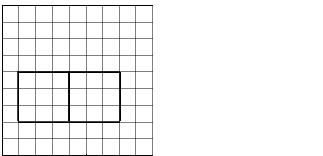
\includegraphics[width=.42\linewidth]{assets/asset-001-01.jpg}
\end{center}
\fillin[{\(\frac{3}{2}\)}]
\begin{solution}
\textbf{答案：}\(\frac{3}{2}\)

\textbf{分析：}首先画出平面区域, 然后将目标函数变形为直线的斜截式, 求在 $y$ 轴的截距最大值.

\textbf{详解：}不等式组表示的平面区域如图阴影部分, 当直线经过 $D$ 点时 $z$ 最大, 由 $\begin{cases}x-2y=0\\x+2y-2=0\end{cases}$ 得 $D(1,\frac{1}{2})$, 所以 $z=x+y$ 的最大值为 $1+\frac{1}{2}=\frac{3}{2}$. 故答案为 $\frac{3}{2}$.
\end{solution}
\end{question}

\begin{question}[points=10]
\textbf{来源：}2016 年 全国III卷-理科，第 24 题\par
[选修4-5：不等式选讲]

已知函数 $f(x)=|2x-a|+a$.

(1) 当 $a=2$ 时, 求不等式 $f(x)\le6$ 的解集;

(2) 设函数 $g(x)=|2x-1|$, 当 $x\in\mathbb{R}$ 时, $f(x)+g(x)\ge3$, 求 $a$ 的取值范围.
\begin{solution}

\textbf{分析：}(1) 当 $a=2$ 时, 由 $|2x-2|+2\le6$, 解绝对值不等式. (2) 由 $f(x)+g(x)=|2x-1|+|2x-a|+a\ge3$, 得 $|x-\frac{1}{2}|+|x-\frac{a}{2}|\ge\frac{3-a}{2}$, 由此能求出 $a$ 的取值范围.

\textbf{详解：}(1) 当 $a=2$ 时, $f(x)=|2x-2|+2$, $\because f(x)\le6$, $\therefore|2x-2|+2\le6$, $|2x-2|\le4$, $|x-1|\le2$, $\therefore-2\le x-1\le2$, 解得 $-1\le x\le3$, $\therefore$ 不等式 $f(x)\le6$ 的解集为 $\{x|-1\le x\le3\}$.
(2) $\because g(x)=|2x-1|$, $\therefore f(x)+g(x)=|2x-1|+|2x-a|+a\ge3$, 即 $2|x-\frac{1}{2}|+2|x-\frac{a}{2}|+a\ge3$, $|x-\frac{1}{2}|+|x-\frac{a}{2}|\ge\frac{3-a}{2}$. 当 $a\ge3$ 时, 成立; 当 $a<3$ 时, $|x-\frac{1}{2}|+|x-\frac{a}{2}|\ge\frac{1}{2}|a-1|$, $\therefore\frac{1}{2}|a-1|\ge\frac{3-a}{2}>0$, 即 $|a-1|\ge3-a$, 两边平方得 $(a-1)^2\ge(3-a)^2$, 解得 $a\ge2$, $\therefore2\le a<3$. 综上, $a$ 的取值范围是 $[2,+\infty)$.
\end{solution}
\end{question}

\begin{question}[points=5]
\textbf{来源：}2016 年 全国III卷-文科，第 13 题\par
设 $x$, $y$ 满足约束条件 $\begin{cases}x-y+1\ge 0\\ x+2y-2\le 0\\ y\ge 0\end{cases}$, 则 $z=2x+3y-5$ 的最小值为 .
\fillin[{$-10$}]
\begin{solution}
\textbf{答案：}$-10$

\textbf{分析：}由约束条件作出可行域, 化目标函数为直线方程的斜截式, 数形结合得到最优解, 联立方程组求得最优解的坐标, 代入目标函数得答案.

\textbf{详解：}由约束条件作出可行域如图, 联立 $\begin{cases}x-y+1=0\\ y=0\end{cases}$, 解得 $A(-1,-1)$. 化目标函数 $z=2x+3y-5$ 为 $y=-\frac{2}{3}x+\frac{z+5}{3}$. 由图可知, 当直线过 $A$ 时, 直线在 $y$ 轴上的截距最小, $z$ 有最小值 $2\times(-1)+3\times(-1)-5=-10$. 故答案为 $-10$.
\end{solution}
\end{question}

\begin{question}[points=10]
\textbf{来源：}2016 年 全国III卷-文科，第 24 题\par
已知函数 $f(x)=|2x-a|+a$.

(1) 当 $a=2$ 时, 求不等式 $f(x)\le 6$ 的解集;

(2) 设函数 $g(x)=|2x-1|$, 当 $x\in\mathbb{R}$ 时, $f(x)+g(x)\ge 3$, 求 $a$ 的取值范围.
\begin{solution}
\textbf{答案：}见解析

\textbf{分析：}(1) 当 $a=2$ 时, 由已知得 $|2x-2|+2\le 6$, 由此能求出不等式 $f(x)\le 6$ 的解集.
(2) 由 $f(x)+g(x)=|2x-1|+|2x-a|+a\ge 3$, 得 $|x-\frac{1}{2}|+|x-\frac{a}{2}|\ge \frac{3-a}{2}$, 由此能求出 $a$ 的取值范围.

\textbf{详解：}(1) 当 $a=2$ 时, $f(x)=|2x-2|+2$, $f(x)\le 6$ 即 $|2x-2|+2\le 6$, $|2x-2|\le 4$, $|x-1|\le 2$, $-2\le x-1\le 2$, 解得 $-1\le x\le 3$. 所以不等式的解集为 $\{x|-1\le x\le 3\}$.
(2) $f(x)+g(x)=|2x-1|+|2x-a|+a\ge 3$ 即 $2|x-\frac{1}{2}|+2|x-\frac{a}{2}|+a\ge 3$, $|x-\frac{1}{2}|+|x-\frac{a}{2}|\ge \frac{3-a}{2}$. 当 $a\ge 3$ 时, 右边 $\le 0$, 不等式恒成立. 当 $a<3$ 时, 左边最小值 $\frac{1}{2}|a-1|\ge \frac{3-a}{2}$ $>0$, 平方得 $(a-1)^2\ge (3-a)^2$, 解得 $a\ge 2$, 所以 $2\le a<3$. 综上, $a$ 的取值范围是 $[2,+\infty)$.
\end{solution}
\end{question}

\begin{question}[points=10]
\textbf{来源：}2016 年 全国II卷-理科，第 24 题\par
已知函数$f(x)=|x-\frac12|+|x+\frac12|$，$M$为不等式$f(x)<2$的解集．

（Ⅰ）求$M$；

（Ⅱ）证明：当$a,b\in M$时，$|a+b|<|1+ab|$．
\begin{solution}
\textbf{答案：}（Ⅰ）$M=(-1,1)$；（Ⅱ）见解析

\textbf{分析：}（Ⅰ）分当$x<-\frac12$时，当$-\frac12\le x\le \frac12$时，当$x>\frac12$时三种情况，分别求解不等式，综合可得答案；（Ⅱ）当$a,b\in M$时，$(a^2-1)(b^2-1)>0$，即$a^2b^2+1>a^2+b^2$，配方后，可证得结论．

\textbf{详解：}（Ⅰ）当$x<-\frac12$时，不等式化为$\frac12-x-x-\frac12<2$，解得$x>-1$，故$-1<x<-\frac12$；当$-\frac12\le x\le \frac12$时，不等式化为$\frac12-x+x+\frac12=1<2$恒成立；当$x>\frac12$时，不等式化为$x-\frac12+x+\frac12<2$，解得$x<1$，故$\frac12<x<1$；综上，$M=(-1,1)$．
（Ⅱ）$a,b\in(-1,1)$，则$a^2<1$，$b^2<1$，所以$(a^2-1)(b^2-1)>0$，即$a^2b^2+1>a^2+b^2$，两边同加$2ab$得$a^2b^2+1+2ab>a^2+b^2+2ab$，即$(ab+1)^2>(a+b)^2$，故$|a+b|<|1+ab|$．
\end{solution}
\end{question}

\begin{question}[points=5]
\textbf{来源：}2016 年 全国II卷-文科，第 14 题\par
若$x$，$y$满足约束条件$\left\{\begin{array}{l}x-y+1\ge0\\ x+y-3\ge0\\ x\le3\end{array}\right.$，则$z=x-2y$的最小值为

\begin{center}
  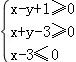
\includegraphics[width=.42\linewidth]{assets/asset-006-01.jpg}
\end{center}
\fillin[{$-5$}]
\begin{solution}
\textbf{答案：}$-5$

\textbf{分析：}可行域端点$(3,4)$，代入$z=3-8=-5$最小。
\end{solution}
\end{question}

\begin{question}[points=10]
\textbf{来源：}2016 年 全国II卷-文科，第 24 题\par
已知函数$f(x)=|x-\frac{1}{2}|+|x+\frac{1}{2}|$，$M$为不等式$f(x)<2$的解集。

（Ⅰ）求$M$；

（Ⅱ）证明：当$a,b\in M$时，$|a+b|<|1+ab|$。
\begin{solution}
\textbf{答案：}（Ⅰ）$(-1,1)$；（Ⅱ）见解析

\textbf{分析：}（Ⅰ）分类讨论得$f(x)<2$的解为$-1<x<1$，即$M=(-1,1)$。
（Ⅱ）$a,b\in(-1,1)$，则$(a^2-1)(b^2-1)>0$，即$a^2b^2+1>a^2+b^2$，两边加$2ab$得$(ab+1)^2>(a+b)^2$，故$|a+b|<|1+ab|$。
\end{solution}
\end{question}

\begin{question}[points=5]
\textbf{来源：}2016 年 全国I卷-理科，第 16 题\par
某高科技企业生产产品$A$和产品$B$需要甲、乙两种新型材料．生产一件产品$A$需要甲材料$1.5kg$，乙材料$1kg$，用$5$个工时；生产一件产品$B$需要甲材料$0.5kg$，乙材料$0.3kg$，用$3$个工时，生产一件产品$A$的利润为$2100$元，生产一件产品$B$的利润为$900$元．该企业现有甲材料$150kg$，乙材料$90kg$，则在不超过$600$个工时的条件下，生产产品$A$、产品$B$的利润之和的最大值为元．
\fillin[{$216000$}]
\begin{solution}
\textbf{答案：}$216000$

\textbf{分析：}设$A$、$B$两种产品分别是$x$件和$y$件，根据题干的等量关系建立不等式组以及目标函数，利用线性规划作出可行域，通过目标函数的几何意义，求出其最大值即可；

\textbf{详解：}解：设$A$、$B$两种产品分别是$x$件和$y$件，获利为$z$元．由题意，得$\begin{cases}1.5x+0.5y\le150\\x+0.3y\le90\\5x+3y\le600\\x\ge0,y\ge0\end{cases}$，$z=2100x+900y$．不等式组表示的可行域如图：由题意可得$\begin{cases}5x+3y=600\\x+0.3y=90\end{cases}$，解得：$\begin{cases}x=60\\y=100\end{cases}$，$A(60,100)$，目标函数$z=2100x+900y$．经过$A$时，直线的截距最大，目标函数取得最大值：$2100\times60+900\times100=216000$元．故答案为：$216000$．
\end{solution}
\end{question}

\begin{question}[points=10]
\textbf{来源：}2016 年 全国I卷-理科，第 24 题\par
已知函数$f(x)=|x+1|-|2x-3|$．

（Ⅰ）在图中画出$y=f(x)$的图象；

（Ⅱ）求不等式$|f(x)|>1$的解集．

\begin{center}
  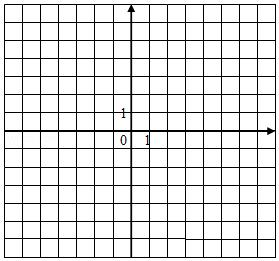
\includegraphics[width=.42\linewidth]{assets/asset-009-01.jpg}
\end{center}
\begin{solution}
\textbf{答案：}（Ⅰ）图象见解析；（Ⅱ）$(-\infty,\frac{1}{3})\cup(1,3)\cup(5,+\infty)$

\textbf{分析：}（Ⅰ）运用分段函数的形式写出$f(x)$的解析式，由分段函数的画法，即可得到所求图象；（Ⅱ）分别讨论当$x\le-1$时，当$-1<x<\frac{3}{2}$时，当$x\ge\frac{3}{2}$时，解绝对值不等式，取交集，最后求并集即可得到所求解集．

\textbf{详解：}解：（Ⅰ）$f(x)=\begin{cases} x-4, & x\le-1 \\ 3x-2, & -1<x<\frac{3}{2} \\ 4-x, & x\ge\frac{3}{2} \end{cases}$，由分段函数的图象画法，可得$f(x)$的图象，如右：（Ⅱ）由$|f(x)|>1$，可得当$x\le-1$时，$|x-4|>1$，解得$x>5$或$x<3$，即有$x\le-1$；当$-1<x<\frac{3}{2}$时，$|3x-2|>1$，解得$x>1$或$x<\frac{1}{3}$，即有$-1<x<\frac{1}{3}$或$1<x<\frac{3}{2}$；当$x\ge\frac{3}{2}$时，$|4-x|>1$，解得$x>5$或$x<3$，即有$x>5$或$\frac{3}{2}\le x<3$．综上可得，$x<\frac{1}{3}$或$1<x<3$或$x>5$．则$|f(x)|>1$的解集为$(-\infty,\frac{1}{3})\cup(1,3)\cup(5,+\infty)$．
\end{solution}
\end{question}

\begin{question}[points=5]
\textbf{来源：}2016 年 全国I卷-文科，第 16 题\par
某高科技企业生产产品$A$和产品$B$需要甲、乙两种新型材料。生产一件产品$A$需要甲材料$1.5\text{kg}$，乙材料$1\text{kg}$，用$5$个工时；生产一件产品$B$需要甲材料$0.5\text{kg}$，乙材料$0.3\text{kg}$，用$3$个工时，生产一件产品$A$的利润为$2100$元，生产一件产品$B$的利润为$900$元。该企业现有甲材料$150\text{kg}$，乙材料$90\text{kg}$，则在不超过$600$个工时的条件下，生产产品$A$、产品$B$的利润之和的最大值为
\fillin[{$216000$}]
\begin{solution}
\textbf{答案：}$216000$

\textbf{分析：}设$A$、$B$两种产品分别是$x$件和$y$件，根据题干的等量关系建立不等式组以及目标函数，利用线性规划作出可行域，通过目标函数的几何意义，求出其最大值即可。

\textbf{详解：}设$A$、$B$两种产品分别是$x$件和$y$件，获利为$z$元。由题意，得$\begin{cases} 1.5x+0.5y\le150 \\ x+0.3y\le90 \\ 5x+3y\le600 \\ x\ge0,y\ge0 \end{cases}$，$z=2100x+900y$。不等式组表示的可行域如图：由题意可得$\begin{cases} x+0.3y=90 \\ 5x+3y=600 \end{cases}$，解得：$\begin{cases} x=60 \\ y=100 \end{cases}$，$A(60,100)$，目标函数$z=2100x+900y$。经过$A$时，直线的截距最大，目标函数取得最大值：$2100\times60+900\times100=216000$元。故答案为：$216000$。
\end{solution}
\end{question}

\begin{question}[points=10]
\textbf{来源：}2016 年 全国I卷-文科，第 24 题\par
[选修4-5：不等式选讲]

已知函数$f(x)=|x+1|-|2x-3|$。

（Ⅰ）在图中画出$y=f(x)$的图象；

（Ⅱ）求不等式$|f(x)|>1$的解集。

\begin{center}
  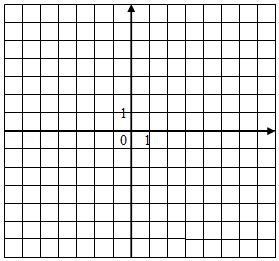
\includegraphics[width=.42\linewidth]{assets/asset-011-01.jpg}
\end{center}
\begin{solution}
\textbf{答案：}（Ⅰ）图象见解析；（Ⅱ）$(-\infty,\frac{1}{3})\cup(1,3)\cup(5,+\infty)$

\textbf{分析：}（Ⅰ）运用分段函数的形式写出$f(x)$的解析式，由分段函数的画法，即可得到所求图象；
（Ⅱ）分别讨论当$x\le-1$时，当$-1<x<\frac{3}{2}$时，当$x\ge\frac{3}{2}$时，解绝对值不等式，取交集，最后求并集即可得到所求解集。

\textbf{详解：}（Ⅰ）$f(x)=\begin{cases} x-4, & x\le-1 \\ 3x-2, & -1<x<\frac{3}{2} \\ 4-x, & x\ge\frac{3}{2} \end{cases}$，由分段函数的图象画法，可得$f(x)$的图象，如右；
（Ⅱ）由$|f(x)|>1$，可得当$x\le-1$时，$|x-4|>1$，解得$x>5$或$x<3$，即有$x\le-1$；当$-1<x<\frac{3}{2}$时，$|3x-2|>1$，解得$x>1$或$x<\frac{1}{3}$，即有$-1<x<\frac{1}{3}$或$1<x<\frac{3}{2}$；当$x\ge\frac{3}{2}$时，$|4-x|>1$，解得$x>5$或$x<3$，即有$x>5$或$\frac{3}{2}\le x<3$。综上可得，$x<\frac{1}{3}$或$1<x<3$或$x>5$。则$|f(x)|>1$的解集为$(-\infty,\frac{1}{3})\cup(1,3)\cup(5,+\infty)$。
\end{solution}
\end{question}

\section*{2017 年}

\begin{question}[points=5]
\textbf{来源：}2017 年 全国III卷-理科，第 13 题\par
若$x$，$y$满足约束条件$\begin{cases} x-y+1\ge 0 \\ x+y-3\le 0 \\ y\ge 0 \end{cases}$，则$z=3x-4y$的最小值为．
\fillin[{$-1$}]
\begin{solution}
\textbf{答案：}$-1$

\textbf{分析：}作出不等式组对应的平面区域，利用目标函数的几何意义，求目标函数$z=3x-4y$的最小值。

\textbf{详解：}由$z=3x-4y$，得$y=\frac{3}{4}x-\frac{z}{4}$，作出不等式对应的可行域（阴影部分），平移直线$y=\frac{3}{4}x-\frac{z}{4}$，由平移可知当直线$y=\frac{3}{4}x-\frac{z}{4}$经过点$B(1,1)$时，直线$y=\frac{3}{4}x-\frac{z}{4}$的截距最大，此时$z$取得最小值，将$B$的坐标代入$z=3x-4y=3-4=-1$，即目标函数$z=3x-4y$的最小值为$-1$。故答案为：$-1$。
\end{solution}
\end{question}

\begin{question}[points=10]
\textbf{来源：}2017 年 全国III卷-理科，第 23 题\par
[选修4-5：不等式选讲]

已知函数$f(x)=|x+1|-|x-2|$．

（1）求不等式$f(x)\ge 1$的解集；

（2）若不等式$f(x)\ge x^2-x+m$的解集非空，求$m$的取值范围．
\begin{solution}
\textbf{答案：}（1）$\{x|x\ge 1\}$；（2）$(-\infty,\frac{5}{4}]$

\textbf{分析：}（1）由于$f(x)=|x+1|-|x-2|=\begin{cases} -3, & x\le -1 \\ 2x-1, & -1<x<2 \\ 3, & x\ge 2 \end{cases}$，解不等式$f(x)\ge 1$可分$-1\le x\le 2$与$x>2$两类讨论即可解得不等式$f(x)\ge 1$的解集；
（2）依题意可得$m\le [f(x)-x^2+x]_{max}$，设$g(x)=f(x)-x^2+x$，分$x\le 1$、$-1<x<2$、$x\ge 2$三类讨论，可求得$g(x)_{max}=\frac{5}{4}$，从而可得$m$的取值范围。

\textbf{详解：}解：（1）因为$f(x)=|x+1|-|x-2|=\begin{cases} -3, & x\le -1 \\ 2x-1, & -1<x<2 \\ 3, & x\ge 2 \end{cases}$，$f(x)\ge 1$，所以当$-1\le x\le 2$时，$2x-1\ge 1$，解得$1\le x\le 2$；当$x>2$时，$3\ge 1$恒成立，故$x>2$；综上，不等式$f(x)\ge 1$的解集为$\{x|x\ge 1\}$．
（2）原式等价于存在$x\in R$使得$f(x)-x^2+x\ge m$成立，即$m\le [f(x)-x^2+x]_{max}$，设$g(x)=f(x)-x^2+x$．由（1）知，$g(x)=\begin{cases} -x^2+x-3, & x\le -1 \\ -x^2+3x-1, & -1<x<2 \\ -x^2+x+3, & x\ge 2 \end{cases}$，当$x\le -1$时，$g(x)=-x^2+x-3$，其开口向下，对称轴方程为$x=\frac{1}{2}>-1$，所以$g(x)\le g(-1)=-1-1-3=-5$；当$-1<x<2$时，$g(x)=-x^2+3x-1$，其开口向下，对称轴方程为$x=\frac{3}{2}\in(-1,2)$，所以$g(x)\le g(\frac{3}{2})=-\frac{9}{4}+\frac{9}{2}-1=\frac{5}{4}$；当$x\ge 2$时，$g(x)=-x^2+x+3$，其开口向下，对称轴方程为$x=\frac{1}{2}<2$，所以$g(x)\le g(2)=-4+2+3=1$；综上，$g(x)_{max}=\frac{5}{4}$，所以$m$的取值范围为$(-\infty,\frac{5}{4}]$。
\end{solution}
\end{question}

\begin{question}[points=5]
\textbf{来源：}2017 年 全国III卷-文科，第 5 题\par
设$x,y$满足约束条件$\begin{cases} x+y-7\le 0 \\ x-3y+1\le 0 \\ 3x-y-5\ge 0 \end{cases}$，则$z=x-y$的取值范围是（      ）

\begin{center}
  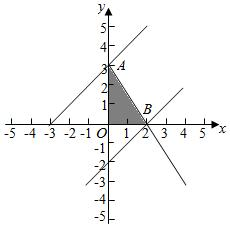
\includegraphics[width=.42\linewidth]{assets/asset-014-01.jpg}
\end{center}
\begin{choices}
  \item A．$[-3,0]$
  \item B．$[-3,2]$
  \item C．$[0,2]$
  \item D．$[0,3]$
\end{choices}
\begin{solution}
\textbf{答案：}B

\textbf{分析：}画出约束条件的可行域，利用目标函数的最优解求解目标函数的范围即可。

\textbf{详解：}可行域如图，由$\begin{cases} x+y-7=0 \\ x-3y+1=0 \end{cases}$得$A(0,3)$，由$\begin{cases} 3x-y-5=0 \\ x-3y+1=0 \end{cases}$得$B(2,0)$，目标函数$z=x-y$在$A$处取最小值$-3$，在$B$处取最大值$2$，故取值范围是$[-3,2]$。
\end{solution}
\end{question}

\begin{question}[points=10]
\textbf{来源：}2017 年 全国III卷-文科，第 23 题\par
[选修4-5：不等式选讲]

已知函数$f(x)=|x+1|-|x-2|$。

（1）求不等式$f(x)\ge 1$的解集；

（2）若不等式$f(x)\ge x^2-x+m$的解集非空，求$m$的取值范围。
\begin{solution}
\textbf{答案：}（1）$\{x|x\ge 1\}$；（2）$(-\infty,\frac{5}{4}]$

\textbf{分析：}（1）分段讨论去绝对值，解不等式。（2）转化为$m\le [f(x)-x^2+x]_{\max}$，求出最大值。

\textbf{详解：}（1）$f(x)=\begin{cases} -3,&x<-1\\ 2x-1,&-1\le x\le 2\\ 3,&x>2 \end{cases}$。$f(x)\ge 1$：当$x<-1$时无解；当$-1\le x\le 2$时，$2x-1\ge 1$得$x\ge 1$；当$x>2$时恒成立。故解集为$\{x|x\ge 1\}$。
（2）设$g(x)=f(x)-x^2+x$，则$g(x)=\begin{cases} -x^2+x-3,&x\le -1\\ -x^2+3x-1,&-1<x<2\\ -x^2+x+3,&x\ge 2 \end{cases}$。分别求得各段最大值：$x\le -1$时最大$g(-1)=-5$；$-1<x<2$时$g(\frac{3}{2})=\frac{5}{4}$；$x\ge 2$时$g(2)=1$。故$g(x)_{\max}=\frac{5}{4}$，所以$m\le \frac{5}{4}$，即$m\in(-\infty,\frac{5}{4}]$。
\end{solution}
\end{question}

\begin{question}[points=5]
\textbf{来源：}2017 年 全国II卷-理科，第 5 题\par
设 $x$，$y$ 满足约束条件 $\begin{cases}2x+3y-3\le 0\\2x-3y+3\ge 0\\y+3\ge 0\end{cases}$，则 $z=2x+y$ 的最小值是（   ）

\begin{center}
  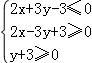
\includegraphics[width=.42\linewidth]{assets/asset-016-01.jpg}
\end{center}
\begin{choices}
  \item $-15$
  \item $-9$
  \item $1$
  \item $9$
\end{choices}
\begin{solution}
\textbf{答案：}$A$

\textbf{分析：}画出约束条件的可行域，利用目标函数的最优解求解目标函数的最小值即可。

\textbf{详解：}$x$、$y$ 满足约束条件的可行域如图：$z=2x+y$ 经过可行域的 $A$ 时，目标函数取得最小值，由 $\begin{cases}2x-3y+3=0\\y+3=0\end{cases}$ 解得 $A(-6,-3)$，则 $z=2x+y$ 的最小值是：$-15$．故选：$A$。
\end{solution}
\end{question}

\begin{question}[points=10]
\textbf{来源：}2017 年 全国II卷-理科，第 23 题\par
[选修4-5：不等式选讲]

已知 $a>0$，$b>0$，$a^3+b^3=2$．证明：

（1）$(a+b)(a^5+b^5)\ge4$；

（2）$a+b\le2$．
\begin{solution}
\textbf{答案：}略

\textbf{分析：}（1）由柯西不等式即可证明，（2）由 $a^3+b^3=2$ 转化为 $\frac{(a+b)^3-2}{3(a+b)}=ab$，再由均值不等式可得：$\frac{(a+b)^3-2}{3(a+b)}=ab\le(\frac{a+b}{2})^2$，即可得到 $\frac{1}{4}(a+b)^3\le2$，问题得以证明。

\textbf{详解：}（1）由柯西不等式得：$(a+b)(a^5+b^5)\ge(\sqrt{a\cdot a^5}+\sqrt{b\cdot b^5})^2=(a^3+b^3)^2\ge4$，当且仅当 $\frac{a}{a^5}=\frac{b}{b^5}$，即 $a=b=1$ 时取等号；
（2）$\because a^3+b^3=2$，$\therefore(a+b)(a^2-ab+b^2)=2$，$\therefore(a+b)[(a+b)^2-3ab]=2$，$\therefore(a+b)^3-3ab(a+b)=2$，$\therefore\frac{(a+b)^3-2}{3(a+b)}=ab$，由均值不等式可得：$\frac{(a+b)^3-2}{3(a+b)}=ab\le(\frac{a+b}{2})^2$，$\therefore(a+b)^3-2\le\frac{3}{4}(a+b)^3$，$\therefore\frac{1}{4}(a+b)^3\le2$，$\therefore a+b\le2$，当且仅当 $a=b=1$ 时等号成立。
\end{solution}
\end{question}

\begin{question}[points=5]
\textbf{来源：}2017 年 全国II卷-文科，第 7 题\par
设 $x$, $y$ 满足约束条件 $\begin{cases} 2x+3y-3\le 0\\ 2x-3y+3\ge 0\\ y+3\ge 0\end{cases}$, 则 $z=2x+y$ 的最小值是
\begin{choices}
  \item $-15$
  \item $-9$
  \item $1$
  \item $9$
\end{choices}
\begin{solution}
\textbf{答案：}$-15$

\textbf{分析：}画出约束条件的可行域, 利用目标函数的最优解求解目标函数的最小值即可.

\textbf{详解：}$x$, $y$ 满足约束条件 $\begin{cases} 2x+3y-3\le 0\\ 2x-3y+3\ge 0\\ y+3\ge 0\end{cases}$ 的可行域如图: $z=2x+y$ 经过可行域的 $A$ 时, 目标函数取得最小值, 由 $\begin{cases} y=-3\\ 2x-3y+3=0\end{cases}$ 解得 $A(-6,-3)$, 则 $z=2x+y$ 的最小值是 $-15$. 故选A.
\end{solution}
\end{question}

\begin{question}[points=10]
\textbf{来源：}2017 年 全国II卷-文科，第 23 题\par
选修4-5: 不等式选讲 \\ 已知 $a>0$, $b>0$, $a^3+b^3=2$. 证明: \\ (1) $(a+b)(a^5+b^5)\ge4$; \\ (2) $a+b\le2$.
\begin{solution}

\textbf{分析：}(1) 由柯西不等式即可证明, (2) 由 $a^3+b^3=2$ 转化为 $\frac{(a+b)^3-2}{3(a+b)}=ab$, 再由均值不等式可得: $\frac{(a+b)^3-2}{3(a+b)}=ab\le\left(\frac{a+b}{2}\right)^2$, 即可得到 $\frac{1}{4}(a+b)^3\le2$, 问题得以证明.

\textbf{详解：}(1) 由柯西不等式得: $(a+b)(a^5+b^5)\ge(\sqrt{a}\cdot\sqrt{a^5}+\sqrt{b}\cdot\sqrt{b^5})^2=(a^3+b^3)^2\ge4$, 当且仅当 $\sqrt{a}\cdot\sqrt{b^5}=\sqrt{b}\cdot\sqrt{a^5}$, 即 $a=b=1$ 时取等号; \\ (2) $\because a^3+b^3=2$, $\therefore (a+b)(a^2-ab+b^2)=2$, $\therefore (a+b)[(a+b)^2-3ab]=2$, $\therefore (a+b)^3-3ab(a+b)=2$, $\therefore \frac{(a+b)^3-2}{3(a+b)}=ab$, 由均值不等式可得: $\frac{(a+b)^3-2}{3(a+b)}=ab\le\left(\frac{a+b}{2}\right)^2$, $\therefore (a+b)^3-2\le\frac{3}{4}(a+b)^3$, $\therefore \frac{1}{4}(a+b)^3\le2$, $\therefore a+b\le2$, 当且仅当 $a=b=1$ 时等号成立.
\end{solution}
\end{question}

\begin{question}[points=5]
\textbf{来源：}2017 年 全国I卷-理科，第 14 题\par
设 $x$，$y$ 满足约束条件 $\begin{cases} x+2y\leq 1 \\ 2x+y\geq -1 \\ x-y\leq 0 \end{cases}$，则 $z=3x-2y$ 的最小值为 ．
\fillin[{$-5$}]
\begin{solution}
\textbf{答案：}$-5$

\textbf{分析：}由约束条件作出可行域，由图得到最优解，求出最优解的坐标，数形结合得答案．

\textbf{详解：}由 $x$，$y$ 满足约束条件 $\begin{cases} x+2y\leq 1 \\ 2x+y\geq -1 \\ x-y\leq 0 \end{cases}$ 作出可行域如图，由图可知，目标函数的最优解为 $A$，联立 $\begin{cases} x+2y=1 \\ x-y=0 \end{cases}$，解得 $A(-1,1)$．所以$z=3x-2y$ 的最小值为 $3\times(-1)-2\times1=-5$．故答案为：$-5$．
\end{solution}
\end{question}

\begin{question}[points=10]
\textbf{来源：}2017 年 全国I卷-理科，第 23 题\par
[选修 4-5：不等式选讲]

已知函数 $f(x)=-x^2+ax+4$，$g(x)=|x+1|+|x-1|$．

（1）当 $a=1$ 时，求不等式 $f(x)\geq g(x)$ 的解集；

（2）若不等式 $f(x)\geq g(x)$ 的解集包含 $[-1,1]$，求 $a$ 的取值范围．
\begin{solution}
\textbf{答案：}（1）$[-1,\frac{\sqrt{17}-1}{2}]$；（2）$[-1,1]$

\textbf{分析：}（1）当 $a=1$ 时，$f(x)=-x^2+x+4$，$g(x)=|x+1|+|x-1|=\begin{cases} -2x, & x\leq-1 \\ 2, & -1<x<1 \\ 2x, & x\geq1 \end{cases}$，分 $x>1$、$x\in[-1,1]$、$x\in(-\infty,-1)$ 三类讨论，结合 $g(x)$ 与 $f(x)$ 的单调性质即可求得 $f(x)\geq g(x)$ 的解集为 $[-1,\frac{\sqrt{17}-1}{2}]$；（2）依题意得：$-x^2+ax+4\geq2$ 在 $[-1,1]$ 恒成立 $\Leftrightarrow x^2-ax-2\leq0$ 在 $[-1,1]$ 恒成立，只需 $\begin{cases} (-1)^2-a(-1)-2\leq0 \\ 1^2-a\cdot1-2\leq0 \end{cases}$，解之即可得 $a$ 的取值范围．

\textbf{详解：}解：（1）当 $a=1$ 时，$f(x)=-x^2+x+4$，是开口向下，对称轴为 $x=\frac{1}{2}$ 的二次函数，$g(x)=|x+1|+|x-1|=\begin{cases} -2x, & x\leq-1 \\ 2, & -1<x<1 \\ 2x, & x\geq1 \end{cases}$，当 $x\in(1,+\infty)$ 时，令 $-x^2+x+4=2x$，解得 $x=\frac{-1+\sqrt{17}}{2}$，$g(x)$ 在 $(1,+\infty)$ 上单调递增，$f(x)$ 在 $(1,+\infty)$ 上单调递减，所以此时 $f(x)\geq g(x)$ 的解集为 $(1,\frac{\sqrt{17}-1}{2}]$；当 $x\in[-1,1]$ 时，$g(x)=2$，$f(x)\geq f(-1)=2$．当 $x\in(-\infty,-1)$ 时，$g(x)$ 单调递减，$f(x)$ 单调递增，且 $g(-1)=f(-1)=2$．综上所述，$f(x)\geq g(x)$ 的解集为 $[-1,\frac{\sqrt{17}-1}{2}]$．
（2）依题意得：$-x^2+ax+4\geq2$ 在 $[-1,1]$ 恒成立，即 $x^2-ax-2\leq0$ 在 $[-1,1]$ 恒成立，则只需 $\begin{cases} (-1)^2-a(-1)-2\leq0 \\ 1^2-a\cdot1-2\leq0 \end{cases}$，解得 $-1\leq a\leq1$，故 $a$ 的取值范围是 $[-1,1]$．
\end{solution}
\end{question}

\begin{question}[points=5]
\textbf{来源：}2017 年 全国I卷-文科，第 7 题\par
设$x$，$y$满足约束条件$\begin{cases} x\ge 0 \\ y\ge 0 \\ x+y\le 3 \end{cases}$，则$z=x+y$的最大值为（   ）
\begin{choices}
  \item 0
  \item 1
  \item 2
  \item 3
\end{choices}
\begin{solution}
\textbf{答案：}D

\textbf{分析：}画出约束条件的可行域，利用目标函数的最优解求解目标函数的最大值即可。

\textbf{详解：}解：$x$，$y$满足约束条件$\begin{cases} x\ge 0 \\ y\ge 0 \\ x+y\le 3 \end{cases}$的可行域如图：$z=x+y$经过可行域的$A$时，目标函数取得最大值，由$\begin{cases} x=3 \\ y=0 \end{cases}$解得$A(3,0)$，所以$z=x+y$的最大值为：3。故选：D。
\end{solution}
\end{question}

\begin{question}[points=10]
\textbf{来源：}2017 年 全国I卷-文科，第 23 题\par
已知函数$f(x)=-x^2+ax+4$，$g(x)=|x+1|+|x-1|$．

（1）当$a=1$时，求不等式$f(x)\ge g(x)$的解集；

（2）若不等式$f(x)\ge g(x)$的解集包含$[-1,1]$，求$a$的取值范围．
\begin{solution}
\textbf{答案：}（1）$[-1,\frac{\sqrt{17}-1}{2}]$；（2）$[-1,1]$。

\textbf{分析：}（1）当$a=1$时，$f(x)=-x^2+x+4$，$g(x)=|x+1|+|x-1|=\begin{cases} 2x, & x>1 \\ 2, & -1\le x\le 1 \\ -2x, & x<-1 \end{cases}$，分$x>1$、$x\in[-1,1]$、$x\in(-\infty,-1)$三类讨论，结合$g(x)$与$f(x)$的单调性质即可求得$f(x)\ge g(x)$的解集为$[-1,\frac{\sqrt{17}-1}{2}]$；（2）依题意得：$-x^2+ax+4\ge2$在$[-1,1]$恒成立$\Leftrightarrow x^2-ax-2\le0$在$[-1,1]$恒成立，只需$\begin{cases} 1-a-2\le0 \\ 1+a-2\le0 \end{cases}$，解之即可得a的取值范围．

\textbf{详解：}解：（1）当$a=1$时，$f(x)=-x^2+x+4$，是开口向下，对称轴为$x=\frac{1}{2}$的二次函数，$g(x)=|x+1|+|x-1|=\begin{cases} 2x, & x>1 \\ 2, & -1\le x\le 1 \\ -2x, & x<-1 \end{cases}$，当$x\in(1,+\infty)$时，令$-x^2+x+4=2x$，解得$x=\frac{\sqrt{17}-1}{2}$，$g(x)$在$(1,+\infty)$上单调递增，$f(x)$在$(1,+\infty)$上单调递减，$\therefore$此时$f(x)\ge g(x)$的解集为$(1,\frac{\sqrt{17}-1}{2}]$；当$x\in[-1,1]$时，$g(x)=2$，$f(x)\ge f(-1)=2$．当$x\in(-\infty,-1)$时，$g(x)$单调递减，$f(x)$单调递增，且$g(-1)=f(-1)=2$．综上所述，$f(x)\ge g(x)$的解集为$[-1,\frac{\sqrt{17}-1}{2}]$；
（2）依题意得：$-x^2+ax+4\ge2$在$[-1,1]$恒成立，即$x^2-ax-2\le0$在$[-1,1]$恒成立，则只需$\begin{cases} (-1)^2-a\cdot(-1)-2\le0 \\ 1^2-a\cdot1-2\le0 \end{cases}$，解得$-1\le a\le1$，故a的取值范围是$[-1,1]$．
\end{solution}
\end{question}

\section*{2018 年}

\begin{question}[points=10]
\textbf{来源：}2018 年 全国III卷-理科，第 23 题\par
设函数$f(x)=|2x+1|+|x-1|$．

（1）画出$y=f(x)$的图象；

（2）当$x\in[0,+\infty)$时，$f(x)\leq ax+b$，求$a+b$的最小值．

\begin{center}
  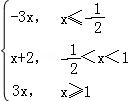
\includegraphics[width=.42\linewidth]{assets/asset-024-01.jpg}
\end{center}
\begin{solution}

\textbf{分析：}（1）利用分段函数的性质将函数表示为分段函数形式进行作图．（2）将不等式恒成立转化为图象关系进行求解．

\textbf{详解：}（1）$f(x)=\begin{cases} -3x, & x\leq -\frac{1}{2} \\ x+2, & -\frac{1}{2}<x<1 \\ 3x, & x\geq 1 \end{cases}$，图象略．
（2）当$x\in[0,+\infty)$时，$f(x)\leq ax+b$恒成立，即$f(x)$的图象在直线$y=ax+b$下方，$x=0$时$f(0)=2\leq b$，$x>0$时，由图象知$a$至少等于$f(x)$在$[0,+\infty)$上各段斜率的最大值3，故$a\geq3$，$b\geq2$，所以$a+b\geq5$，当$a=3$，$b=2$时取等，故$a+b$的最小值为5．
\end{solution}
\end{question}

\begin{question}[points=5]
\textbf{来源：}2018 年 全国III卷-文科，第 15 题\par
若变量 $x,y$ 满足约束条件 $\begin{cases} 2x+y+3\ge 0 \\ x-2y+4\ge 0 \\ x-2\le 0 \end{cases}$，则 $z=x+\frac{1}{3}y$ 的最大值是
\fillin[{$3$}]
\begin{solution}
\textbf{答案：}$3$

\textbf{分析：}作出不等式组表示的平面区域；作出目标函数对应的直线；结合图象知当直线过 $(2,3)$ 时，$z$ 最大．

\textbf{详解：}画出变量 $x,y$ 满足约束条件 $\begin{cases} 2x+y+3\ge 0 \\ x-2y+4\ge 0 \\ x-2\le 0 \end{cases}$ 表示的平面区域如图：由 $\begin{cases} x=2 \\ x-2y+4=0 \end{cases}$ 解得 $A(2,3)$．$z=x+\frac{1}{3}y$ 变形为 $y=-3x+3z$，作出目标函数对应的直线，当直线过 $A(2,3)$ 时，直线的纵截距最小，$z$ 最大，最大值为 $2+\frac{1}{3}\times 3=3$．故答案为：$3$．
\end{solution}
\end{question}

\begin{question}[points=10]
\textbf{来源：}2018 年 全国III卷-文科，第 23 题\par
[选修 4-5：不等式选讲]（10 分）

设函数 $f(x)=|2x+1|+|x-1|$．

(1) 画出 $y=f(x)$ 的图象；

(2) 当 $x\in[0,+\infty)$ 时，$f(x)\le ax+b$，求 $a+b$ 的最小值．

\begin{center}
  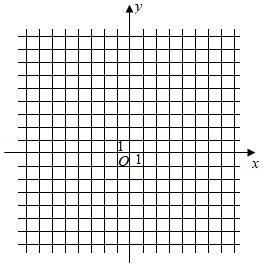
\includegraphics[width=.42\linewidth]{assets/asset-026-01.jpg}
\end{center}

\begin{center}
  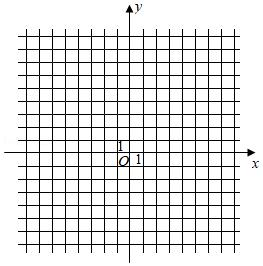
\includegraphics[width=.42\linewidth]{assets/asset-026-02.jpg}
\end{center}
\begin{solution}

\textbf{分析：}(1) 利用分段函数的性质将函数表示为分段函数形式进行作图即可．
(2) 将不等式恒成立转化为图象关系进行求解即可．

\textbf{详解：}(1) 当 $x\le -\frac{1}{2}$ 时，$f(x)=-(2x+1)-(x-1)=-3x$；当 $-\frac{1}{2}<x<1$ 时，$f(x)=(2x+1)-(x-1)=x+2$；当 $x\ge 1$ 时，$f(x)=(2x+1)+(x-1)=3x$．则 $f(x)=\begin{cases} -3x, & x\le -\frac{1}{2} \\ x+2, & -\frac{1}{2}<x<1 \\ 3x, & x\ge 1 \end{cases}$，图象略．
(2) 当 $x\in[0,+\infty)$ 时，$f(x)\le ax+b$，当 $x=0$ 时，$f(0)=2\le 0\cdot a+b$，$\therefore b\ge 2$；当 $x>0$ 时，要使 $f(x)\le ax+b$ 恒成立，则函数 $f(x)$ 的图象都在直线 $y=ax+b$ 的下方或在直线上，$\because f(x)$ 的图象与 $y$ 轴的交点的纵坐标为 $2$，且各部分直线的斜率的最大值为 $3$，故当且仅当 $a\ge 3$ 且 $b\ge 2$ 时，不等式 $f(x)\le ax+b$ 在 $[0,+\infty)$ 上成立，$\therefore a+b$ 的最小值为 $5$．
\end{solution}
\end{question}

\begin{question}[points=5]
\textbf{来源：}2018 年 全国II卷-理科，第 14 题\par
若$x,y$满足约束条件$\begin{cases} x+2y-5\ge 0 \\ x-2y+3\ge 0 \\ x-5\le 0 \end{cases}$，则$z=x+y$的最大值为      ．
\fillin[{$9$}]
\begin{solution}
\textbf{答案：}$9$

\textbf{分析：}由约束条件作出可行域，数形结合得到最优解，求出最优解的坐标，代入目标函数得答案．

\textbf{详解：}由约束条件作出可行域如图，化目标函数$z=x+y$为$y=-x+z$，由图可知，当直线$y=-x+z$过$A$时，$z$取得最大值，由$\begin{cases} x=5 \\ x-2y+3=0 \end{cases}$，解得$A(5,4)$，目标函数有最大值，为$z=9$．
\end{solution}
\end{question}

\begin{question}[points=10]
\textbf{来源：}2018 年 全国II卷-理科，第 23 题\par
[选修4-5：不等式选讲]

设函数$f(x)=5-|x+a|-|x-2|$．

（1）当$a=1$时，求不等式$f(x)\ge 0$的解集；

（2）若$f(x)\le 1$，求$a$的取值范围．
\begin{solution}

\textbf{分析：}（1）去绝对值，化为分段函数，求出不等式的解集即可，
（2）由题意可得$|x+a|+|x-2|\ge 4$，根据绝对值的几何意义即可求出．

\textbf{详解：}（1）当$a=1$时，$f(x)=5-|x+1|-|x-2|=\begin{cases} 2x+4, & x\le -1 \\ 2, & -1<x<2 \\ -2x+6, & x\ge 2 \end{cases}$．当$x\le -1$时，$f(x)=2x+4\ge0$，解得$-2\le x\le -1$；当$-1<x<2$时，$f(x)=2\ge0$恒成立，即$-1<x<2$；当$x\ge2$时，$f(x)=-2x+6\ge0$，解得$2\le x\le 3$．综上所述不等式$f(x)\ge0$的解集为$[-2,3]$．
（2）$\because f(x)\le1$，$\therefore5-|x+a|-|x-2|\le1$，$\therefore|x+a|+|x-2|\ge4$，$\because|x+a|+|x-2|=|x+a|+|2-x|\ge|x+a+2-x|=|a+2|$，$\therefore|a+2|\ge4$，解得$a\le -6$或$a\ge2$，故$a$的取值范围为$(-\infty,-6]\cup[2,+\infty)$．
\end{solution}
\end{question}

\begin{question}[points=5]
\textbf{来源：}2018 年 全国II卷-文科，第 14 题\par
若 $x$，$y$ 满足约束条件 $\begin{cases} x+2y-5\leq0 \\ 2x+y-7\leq0 \\ x\geq0,y\geq0 \end{cases}$，则 $z=x+y$ 的最大值为

\begin{center}
  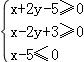
\includegraphics[width=.42\linewidth]{assets/asset-029-01.jpg}
\end{center}
\fillin[{$9$}]
\begin{solution}
\textbf{答案：}$9$

\textbf{分析：}由约束条件作出可行域，数形结合得到最优解，求出最优解的坐标，代入目标函数得答案。

\textbf{详解：}由约束条件作出可行域，化目标函数 $z=x+y$ 为 $y=-x+z$，由图可知，当直线 $y=-x+z$ 过 $A$ 时，$z$ 取得最大值，由 $\begin{cases} x+2y-5=0 \\ 2x+y-7=0 \end{cases}$ 解得 $A(5,4)$，目标函数有最大值，为 $z=9$。故答案为：$9$。
\end{solution}
\end{question}

\begin{question}[points=10]
\textbf{来源：}2018 年 全国II卷-文科，第 23 题\par
[选修4-5：不等式选讲]（10分）

设函数 $f(x)=5-|x+a|-|x-2|$。

（1）当 $a=1$ 时，求不等式 $f(x)\geq0$ 的解集；

（2）若 $f(x)\leq1$，求 $a$ 的取值范围。
\begin{solution}

\textbf{分析：}（1）去绝对值，化为分段函数，求出不等式的解集即可；
（2）由题意可得 $|x+a|+|x-2|\geq4$，根据绝对值的几何意义即可求出。

\textbf{详解：}（1）当 $a=1$ 时，$f(x)=5-|x+1|-|x-2|=\begin{cases} 2x+4, & x\leq-1 \\ 2, & -1<x<2 \\ -2x+6, & x\geq2 \end{cases}$，当 $x\leq-1$ 时，$f(x)=2x+4\geq0$，解得 $-2\leq x\leq-1$；当 $-1<x<2$ 时，$f(x)=2\geq0$ 恒成立，即 $-1<x<2$；当 $x\geq2$ 时，$f(x)=-2x+6\geq0$，解得 $2\leq x\leq3$，综上所述不等式 $f(x)\geq0$ 的解集为 $[-2,3]$。
（2）因为$f(x)\leq1$，所以$5-|x+a|-|x-2|\leq1$，所以$|x+a|+|x-2|\geq4$，又 $|x+a|+|x-2|=|x+a|+|2-x|\geq|x+a+2-x|=|a+2|$，所以$|a+2|\geq4$，解得 $a\leq-6$ 或 $a\geq2$，故 $a$ 的取值范围是 $(-\infty,-6]\cup[2,+\infty)$。
\end{solution}
\end{question}

\begin{question}[points=5]
\textbf{来源：}2018 年 全国I卷-理科，第 13 题\par
若$x$，$y$满足约束条件$\begin{cases} x-2y-2\leq0 \\ x-y+1\geq0 \\ y\leq0 \end{cases}$，则$z=3x+2y$的最大值为。
\fillin[{$6$}]
\begin{solution}
\textbf{答案：}$6$

\textbf{分析：}作出不等式组对应的平面区域，利用目标函数的几何意义进行求解即可。

\textbf{详解：}作出不等式组对应的平面区域（图略），由$z=3x+2y$得$y=-\frac{3}{2}x+\frac{z}{2}$，平移直线，当经过点$A(2,0)$时，直线的截距最大，此时$z$最大，最大值为$z=3\times2=6$。
\end{solution}
\end{question}

\begin{question}[points=10]
\textbf{来源：}2018 年 全国I卷-理科，第 23 题\par
已知$f(x)=|x+1|-|ax-1|$。

（1）当$a=1$时，求不等式$f(x)>1$的解集；

（2）若$x\in(0,1)$时不等式$f(x)>x$成立，求$a$的取值范围。
\begin{solution}

\textbf{分析：}（1）去绝对值，化为分段函数，即可求出不等式的解集。（2）当$x\in(0,1)$时不等式$f(x)>x$成立，转化为$|ax-1|<1$，即$0<ax<2$，转化为$a<\frac{2}{x}$，即可求出$a$的范围。

\textbf{详解：}（1）当$a=1$时，$f(x)=|x+1|-|x-1|=\begin{cases} -2, & x\leq-1 \\ 2x, & -1<x<1 \\ 2, & x\geq1 \end{cases}$。由$f(x)>1$得，当$x\leq-1$时，$-2>1$不成立；当$-1<x<1$时，$2x>1$，解得$x>\frac{1}{2}$；当$x\geq1$时，$2>1$恒成立。综上，解集为$(\frac{1}{2},+\infty)$。
（2）当$x\in(0,1)$时，$x+1>0$，$ax-1$符号不定。$f(x)>x$即$|x+1|-|ax-1|>x$，$\because x+1>x$，$\therefore |ax-1|<1$，即$-1<ax-1<1$，$0<ax<2$。$\because x\in(0,1)$，$\therefore a>0$，且$a<\frac{2}{x}$对$x\in(0,1)$恒成立，$\because \frac{2}{x}>2$，$\therefore a\leq2$。综上，$a$的取值范围为$(0,2]$。
\end{solution}
\end{question}

\begin{question}[points=5]
\textbf{来源：}2018 年 全国I卷-文科，第 14 题\par
若 $x,y$ 满足约束条件 $\begin{cases} x-2y-2\le 0 \\ x-y+1\ge 0 \\ y\le 0 \end{cases}$，则 $z=3x+2y$ 的最大值为

\begin{center}
  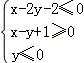
\includegraphics[width=.42\linewidth]{assets/asset-033-01.jpg}
\end{center}
\fillin[{$6$}]
\begin{solution}
\textbf{答案：}$6$

\textbf{分析：}作出不等式组对应的平面区域，利用目标函数的几何意义进行求解即可。

\textbf{详解：}作出不等式组对应的平面区域如图：由 $z=3x+2y$ 得 $y=-\frac{3}{2}x+\frac{z}{2}$，平移直线 $y=-\frac{3}{2}x+\frac{z}{2}$，由图象知当直线经过点 $A(2,0)$ 时，直线的截距最大，此时 $z$ 最大，最大值为 $z=3\times2=6$。故答案为：$6$。
\end{solution}
\end{question}

\begin{question}[points=10]
\textbf{来源：}2018 年 全国I卷-文科，第 23 题\par
[选修 4-5：不等式选讲]（10 分）

已知 $f(x)=|x+1|-|ax-1|$。

（1）当 $a=1$ 时，求不等式 $f(x)>1$ 的解集；

（2）若 $x\in(0,1)$ 时不等式 $f(x)>x$ 成立，求 $a$ 的取值范围。
\begin{solution}

\textbf{分析：}（1）去绝对值，化为分段函数，即可求出不等式的解集。（2）当 $x\in(0,1)$ 时不等式 $f(x)>x$ 成立，转化为 $|ax-1|<1$，即 $0<ax<2$，进一步求解。

\textbf{详解：}（1）当 $a=1$ 时，$f(x)=|x+1|-|x-1|=\begin{cases} -2, & x<-1 \\ 2x, & -1\le x\le 1 \\ 2, & x>1 \end{cases}$，由 $f(x)>1$，得 $\begin{cases} -1\le x\le 1 \\ 2x>1 \end{cases}$ 或 $\begin{cases} x>1 \\ 2>1 \end{cases}$，解得 $x>\frac{1}{2}$，故不等式 $f(x)>1$ 的解集为 $(\frac{1}{2},+\infty)$。
（2）当 $x\in(0,1)$ 时，$f(x)>x$ 即 $|x+1|-|ax-1|>x$，由于 $x+1>0$，则 $x+1-|ax-1|>x$，即 $|ax-1|<1$，$\therefore -1<ax-1<1$，$\therefore 0<ax<2$，$\because x\in(0,1)$，$\therefore a>0$，$\therefore 0<x<\frac{2}{a}$，$\therefore \frac{2}{a}>1$，$\therefore a<2$，又 $a>0$，故 $a$ 的取值范围为 $(0,2]$。
\end{solution}
\end{question}

\section*{2019 年}

\begin{question}[points=10]
\textbf{来源：}2019 年 全国III卷-理科，第 23 题\par
[选修 4-5：不等式选讲]（10 分）

设 $x,y,z\in\mathbb{R}$，且 $x+y+z=1$。

（1）求 $(x-1)^2+(y+1)^2+(z+1)^2$ 的最小值；

（2）若 $(x-2)^2+(y-1)^2+(z-a)^2\ge\dfrac{1}{3}$ 成立，证明：$a\le -3$ 或 $a\ge -1$。
\begin{solution}
\textbf{答案：}（1）$\dfrac{4}{3}$；（2）见详解。

\textbf{分析：}(1)根据条件 $x+y+z=1$ 和柯西不等式得到最小值，再讨论是否达到等号。(2)利用柯西不等式得到 $a$ 的范围。

\textbf{详解：}（2）由柯西不等式得 $[(x-2)^2+(y-1)^2+(z-a)^2](1^2+1^2+1^2) \ge [(x-2)+(y-1)+(z-a)]^2 = (x+y+z-3-a)^2 = (a+2)^2$，当且仅当 $x-2=y-1=z-a$ 时等号成立。故 $(x-2)^2+(y-1)^2+(z-a)^2$ 的最小值为 $\dfrac{(a+2)^2}{3}$。由题设知 $\dfrac{(a+2)^2}{3} \ge \dfrac{1}{3}$，即 $(a+2)^2 \ge 1$，解得 $a\le -3$ 或 $a\ge -1$。
\end{solution}
\end{question}

\begin{question}[points=10]
\textbf{来源：}2019 年 全国III卷-文科，第 23 题\par
[选修4-5：不等式选讲]（10分）

设$x,y,z\in\mathbf{R}$，且$x+y+z=1$。

(1)求$(x-1)^2+(y+1)^2+(z+1)^2$的最小值；

(2)若$(x-2)^2+(y-1)^2+(z-a)^2\ge\frac{1}{3}$成立，证明：$a\le-3$或$a\ge-1$。
\begin{solution}
\textbf{答案：}(1) $\frac{4}{3}$; (2)见详解

\textbf{分析：}(1)根据条件$x+y+z=1$，和柯西不等式得到$(x-1)^2+(y+1)^2+(z+1)^2\ge\frac{4}{3}$，再讨论$x,y,z$是否可以达到等号成立的条件。(2)恒成立问题，柯西不等式等号成立时构造的$x,y,z$代入原不等式，便可得到参数的取值范围。

\textbf{详解：}(1) $[(x-1)^2+(y+1)^2+(z+1)^2](1^2+1^2+1^2)\ge[(x-1)+(y+1)+(z+1)]^2=(x+y+z+1)^2=4$，故$(x-1)^2+(y+1)^2+(z+1)^2\ge\frac{4}{3}$。等号成立当且仅当$x-1=y+1=z+1$，而又因$x+y+z=1$，解得$\begin{cases}x=\frac{5}{3}\\y=-\frac{1}{3}\\z=-\frac{1}{3}\end{cases}$时等号成立。所以$(x-1)^2+(y+1)^2+(z+1)^2$的最小值为$\frac{4}{3}$。
(2)因为$(x-2)^2+(y-1)^2+(z-a)^2\ge\frac{1}{3}$，所以$[(x-2)^2+(y-1)^2+(z-a)^2](1^2+1^2+1^2)\ge1$。根据柯西不等式等号成立条件，当$x-2=y-1=z-a$，即$\begin{cases}x=2-\frac{a+2}{3}\\y=1-\frac{a+2}{3}\\z=a-\frac{a+2}{3}\end{cases}$时有$[(x-2)^2+(y-1)^2+(z-a)^2](1^2+1^2+1^2)=(x-2+y-1+z-a)^2=(a+2)^2$成立。所以$(a+2)^2\ge1$成立，所以有$a\le-3$或$a\ge-1$。
另解：用反证法。若$a\le-3$或$a\ge-1$不成立，那么$-1<a<3$成立，则$(a+2)^2<1$。而$[(x-2)^2+(y-1)^2+(z-a)^2](1^2+1^2+1^2)=(x-2+y-1+z-a)^2$左面等号成立当且仅当$x-2=y-1=z-a$，又因为$x+y+z=1$，所以$x-2=y-1=z-a=-\frac{a+2}{3}$。故此时$[(x-2)^2+(y-1)^2+(z-a)^2](1^2+1^2+1^2)=(x-2+y-1+z-a)^2=(a+2)^2<1$，即$(x-2)^2+(y-1)^2+(z-a)^2<\frac{1}{3}$，与原命题矛盾。
\end{solution}
\end{question}

\begin{question}[points=5]
\textbf{来源：}2019 年 全国II卷-理科，第 6 题\par
若 $a>b$，则
\begin{choices}
  \item $\ln(a-b)>0$
  \item $3^a<3^b$
  \item $a^3-b^3>0$
  \item $|a|>|b|$
\end{choices}
\begin{solution}
\textbf{答案：}$C$

\textbf{分析：}本题也可用直接法，因为 $a>b$，所以 $a-b>0$，当 $a-b=1$ 时，$\ln(a-b)=0$，知 $A$ 错；因为 $y=3^x$ 是增函数，所以 $3^a>3^b$，故 $B$ 错；因为幂函数 $y=x^3$ 是增函数，$a>b$，所以 $a^3>b^3$，知 $C$ 正确；取 $a=1,b=-2$，满足 $a>b$，$1=|a|<|b|=2$，知 $D$ 错．

\textbf{详解：}取 $a=2,b=1$，满足 $a>b$，$\ln(a-b)=0$，知 $A$ 错；因为 $9=3^a>3^b=3$，知 $B$ 错；取 $a=1,b=-2$，满足 $a>b$，$1=|a|<|b|=2$，知 $D$ 错；因为幂函数 $y=x^3$ 是增函数，$a>b$，所以 $a^3>b^3$，故选 $C$．
\end{solution}
\end{question}

\begin{question}[points=10]
\textbf{来源：}2019 年 全国II卷-理科，第 23 题\par
[选修 4-5：不等式选讲]（10 分）

已知 $f(x)=|x-a|x+|x-2|(x-a)$．

（1）当 $a=1$ 时，求不等式 $f(x)<0$ 的解集；

（2）若 $x\in(-\infty,1)$ 时，$f(x)<0$，求 $a$ 的取值范围．
\begin{solution}
\textbf{答案：}（1）$(-\infty,1)$；（2）$[1,+\infty)$

\textbf{分析：}（1）根据 $a=1$，将原不等式化为 $|x-1|x+|x-2|(x-1)<0$，分别讨论 $x<1$，$1\leq x<2$，$x\geq 2$ 三种情况，即可求出结果；（2）分别讨论 $a\geq 1$ 和 $a<1$ 两种情况，即可得出结果．

\textbf{详解：}（1）当 $a=1$ 时，原不等式可化为 $|x-1|x+|x-2|(x-1)<0$．当 $x<1$ 时，原不等式可化为 $(1-x)x+(2-x)(x-1)<0$，即 $(x-1)^2>0$，显然成立，此时解集为 $(-\infty,1)$；当 $1\leq x<2$ 时，原不等式可化为 $(x-1)x+(2-x)(x-1)<0$，解得 $x<1$，此时解集为空集；当 $x\geq 2$ 时，原不等式可化为 $(x-1)x+(x-2)(x-1)<0$，即 $(x-1)^2<0$，显然不成立，此时解集为空集．综上，原不等式的解集为 $(-\infty,1)$．
（2）当 $a\geq 1$ 时，因为 $x\in(-\infty,1)$，所以由 $f(x)<0$ 可得 $(a-x)x+(2-x)(x-a)<0$，即 $(x-a)(x-1)>0$，显然恒成立；所以 $a\geq 1$ 满足题意．当 $a<1$ 时，$f(x)=\begin{cases} 2(x-a), & a\leq x<1 \\ 2(x-a)(1-x), & x<a \end{cases}$，因为 $a\leq x<1$ 时，$f(x)<0$ 显然不能成立，所以 $a<1$ 不满足题意．综上，$a$ 的取值范围是 $[1,+\infty)$．
\end{solution}
\end{question}

\begin{question}[points=5]
\textbf{来源：}2019 年 全国II卷-文科，第 13 题\par
若变量 $x,y$ 满足约束条件 $\begin{cases}2x+3y-6\ge 0,\\ x+y-3\le 0,\\ y-2\le 0,\end{cases}$ 则 $z=3x-y$ 的最大值是.
\fillin[{$9$}]
\begin{solution}
\textbf{答案：}$9$

\textbf{分析：}作出可行域，平移 $3x-y=0$ 找到目标函数取到最大值的点，求出点的坐标，代入目标函数可得．

\textbf{详解：}画出不等式组表示的可行域，阴影部分表示的三角形 $ABC$ 区域，根据直线 $3x-y-z=0$ 中的 $z$ 表示纵截距的相反数，当直线 $z=3x-y$ 过点 $C(3,0)$ 时，$z$ 取最大值为 $9$．
\end{solution}
\end{question}

\begin{question}[points=10]
\textbf{来源：}2019 年 全国II卷-文科，第 23 题\par
[选修 4-5：不等式选讲]

已知 $f(x)=|x-a|x+|x-2|(x-a)$．

（1）当 $a=1$ 时，求不等式 $f(x)<0$ 的解集；

（2）若 $x\in(-\infty,1)$ 时，$f(x)<0$，求 $a$ 的取值范围．
\begin{solution}
\textbf{答案：}（1）$(-\infty,1)$；（2）$[1,+\infty)$

\textbf{分析：}（1）根据 $a=1$，将原不等式化为 $|x-1|x+|x-2|(x-1)<0$，分别讨论 $x<1$，$1\le x<2$，$x\ge2$ 三种情况，即可求出结果；
（2）分别讨论 $a\ge1$ 和 $a<1$ 两种情况，即可得出结果．

\textbf{详解：}（1）当 $a=1$ 时，原不等式可化为 $|x-1|x+|x-2|(x-1)<0$；当 $x<1$ 时，原不等式可化为 $(1-x)x+(2-x)(x-1)<0$，即 $(x-1)^2>0$，显然成立，此时解集为 $(-\infty,1)$；当 $1\le x<2$ 时，原不等式可化为 $(x-1)x+(2-x)(x-1)<0$，解得 $x<1$，此时解集为空集；当 $x\ge2$ 时，原不等式可化为 $(x-1)x+(x-2)(x-1)<0$，即 $(x-1)^2<0$，显然不成立；此时解集为空集；综上，原不等式的解集为 $(-\infty,1)$．
（2）当 $a\ge1$ 时，因为 $x\in(-\infty,1)$，所以由 $f(x)<0$ 可得 $(a-x)x+(2-x)(x-a)<0$，即 $(x-a)(x-1)>0$，显然恒成立；所以 $a\ge1$ 满足题意；当 $a<1$ 时，$f(x)=\begin{cases}2(x-a), & a\le x<1 \\ 2(x-a)(1-x), & x<a\end{cases}$，因为 $a\le x<1$ 时，$f(x)<0$ 显然不能成立，所以 $a<1$ 不满足题意；综上，$a$ 的取值范围是 $[1,+\infty)$．
\end{solution}
\end{question}

\begin{question}[points=10]
\textbf{来源：}2019 年 全国I卷-理科，第 23 题\par
[选修 4—5：不等式选讲]

已知 $a$, $b$, $c$ 为正数，且满足 $abc = 1$．证明：

(1) $\frac{1}{a} + \frac{1}{b} + \frac{1}{c} \le a^2 + b^2 + c^2$;

(2) $(a + b)^3 + (b + c)^3 + (c + a)^3 \ge 24$．
\begin{solution}
\textbf{答案：}见解析

\textbf{分析：}(1) 利用 $abc = 1$ 将所证不等式可变为证明：$a^2 + b^2 + c^2 \ge bc + ac + ab$，利用基本不等式可证得 $2(a^2 + b^2 + c^2) \ge 2ab + 2bc + 2ac$，从而得到结论；(2) 利用基本不等式可得 $(a+b)^3 + (b+c)^3 + (c+a)^3 \ge 3(a+b)(b+c)(c+a)$，再次利用基本不等式可将式转化为 $(a+b)^3 + (b+c)^3 + (c+a)^3 \ge 24(abc)^2$，在取等条件一致的情况下，可得结论．

\textbf{详解：}(1) $\because abc = 1$, $\therefore \frac{1}{a} + \frac{1}{b} + \frac{1}{c} = \left(\frac{1}{a} + \frac{1}{b} + \frac{1}{c}\right) \cdot abc = bc + ac + ab$．$\because 2(a^2 + b^2 + c^2) = (a^2 + b^2) + (b^2 + c^2) + (c^2 + a^2) \ge 2ab + 2bc + 2ac$, 当且仅当 $a = b = c$ 时取等号，$\therefore 2(a^2 + b^2 + c^2) \ge 2(ab + bc + ac)$, 即 $a^2 + b^2 + c^2 \ge ab + bc + ac = \frac{1}{a} + \frac{1}{b} + \frac{1}{c}$．
(2) $\because (a+b)^3 + (b+c)^3 + (c+a)^3 \ge 3(a+b)(b+c)(c+a)$, 当且仅当 $a = b = c$ 时取等号．又 $a+b \ge 2\sqrt{ab}$, $b+c \ge 2\sqrt{bc}$, $a+c \ge 2\sqrt{ac}$ (当且仅当 $a = b = c$ 时等号同时成立)，$\therefore (a+b)^3 + (b+c)^3 + (c+a)^3 \ge 3 \times 2\sqrt{ab} \times 2\sqrt{bc} \times 2\sqrt{ac} = 24(abc)^2 = 24$．
\end{solution}
\end{question}

\begin{question}[points=10]
\textbf{来源：}2019 年 全国I卷-文科，第 23 题\par
已知 $a$，$b$，$c$ 为正数，且满足 $abc=1$．证明：

（1）$\frac{1}{a} + \frac{1}{b} + \frac{1}{c} \le a^2 + b^2 + c^2$；

（2）$(a+b)^3 + (b+c)^3 + (c+a)^3 \ge 24$．
\begin{solution}
\textbf{答案：}见解析。

\textbf{分析：}（1）利用 $abc=1$ 将所证不等式可变为证明 $a^2+b^2+c^2 \ge bc+ac+ab$，利用基本不等式可证得 $2(a^2+b^2+c^2) \ge 2ab+2bc+2ac$，从而得到结论；（2）利用基本不等式可得 $(a+b)^3+(b+c)^3+(c+a)^3 \ge 3(a+b)(b+c)(c+a)$，再次利用基本不等式可将式子转化为 $(a+b)^3+(b+c)^3+(c+a)^3 \ge 24(abc)^2$，结合 $abc=1$ 可得结论。

\textbf{详解：}（1）因为 $abc=1$，所以 $\frac{1}{a}+\frac{1}{b}+\frac{1}{c} = (\frac{1}{a}+\frac{1}{b}+\frac{1}{c})\cdot abc = bc+ac+ab$，而 $2(a^2+b^2+c^2) = (a^2+b^2)+(b^2+c^2)+(c^2+a^2) \ge 2ab+2bc+2ac$，当且仅当 $a=b=c$ 时取等号，所以 $2(a^2+b^2+c^2) \ge 2(\frac{1}{a}+\frac{1}{b}+\frac{1}{c})$，即 $a^2+b^2+c^2 \ge \frac{1}{a}+\frac{1}{b}+\frac{1}{c}$。
（2）因为 $(a+b)^3+(b+c)^3+(c+a)^3 \ge 3\sqrt[3]{(a+b)^3(b+c)^3(c+a)^3} = 3(a+b)(b+c)(c+a)$，当且仅当 $a=b=c$ 时取等号，又 $a+b \ge 2\sqrt{ab}$，$b+c \ge 2\sqrt{bc}$，$a+c \ge 2\sqrt{ac}$（当且仅当 $a=b=c$ 时等号同时成立），所以 $(a+b)^3+(b+c)^3+(c+a)^3 \ge 3 \times 2\sqrt{ab} \times 2\sqrt{bc} \times 2\sqrt{ac} = 24(abc)^2 = 24$。
\end{solution}
\end{question}

\section*{2020 年}

\begin{question}[points=5]
\textbf{来源：}2020 年 全国III卷-理科，第 13 题\par
若 $x,y$ 满足约束条件 $\begin{cases} x+y\ge0 \\ 2x-y\ge0 \\ x\le1 \end{cases}$，则 $z=3x+2y$ 的最大值为 。
\fillin[{$7$}]
\begin{solution}
\textbf{答案：}$7$

\textbf{分析：}作出可行域，利用线性规划求解。

\textbf{详解：}作出可行域如图。由 $z=3x+2y$ 得 $y=-\frac32x+\frac{z}{2}$，当直线经过点 $A$ 时截距最大，$z$ 最大。解 $\begin{cases} y=2x \\ x=1 \end{cases}$ 得 $A(1,2)$，所以 $z_{\max}=3\times1+2\times2=7$。
\end{solution}
\end{question}

\begin{question}[points=10]
\textbf{来源：}2020 年 全国III卷-理科，第 23 题\par
[选修4-5：不等式选讲]

设 $a,b,c\in\mathbb{R}$，$a+b+c=0$，$abc=1$。

(1) 证明：$ab+bc+ca<0$；

(2) 用 $\max\{a,b,c\}$ 表示 $a,b,c$ 的最大值，证明：$\max\{a,b,c\}\ge\sqrt[3]{4}$。
\begin{solution}
\textbf{答案：}见解析

\textbf{分析：}(1) 利用 $(a+b+c)^2=0$ 展开得 $ab+bc+ca=-\frac12(a^2+b^2+c^2)<0$；(2) 不妨设 $a$ 最大，利用 $a+b+c=0$ 和 $abc=1$ 得 $a>0,b,c<0$，然后利用基本不等式。

\textbf{详解：}(1) 因为 $(a+b+c)^2=a^2+b^2+c^2+2(ab+bc+ca)=0$，所以 $ab+bc+ca=-\frac12(a^2+b^2+c^2)$。由于 $a,b,c$ 不全为 $0$，$a^2+b^2+c^2>0$，故 $ab+bc+ca<0$。
(2) 不妨设 $a=\max\{a,b,c\}$，由 $a+b+c=0$，$abc=1$ 知 $a>0$，$b<0$，$c<0$。由 $a+b+c=0$ 得 $b+c=-a$，$bc=\frac1a$。则 $a^3=a^2\cdot a=(b+c)^2\cdot a=(b^2+c^2+2bc)a\ge (2bc+2bc)a=4abc=4$（当且仅当 $b=c$ 时取等），所以 $a\ge\sqrt[3]{4}$，即 $\max\{a,b,c\}\ge\sqrt[3]{4}$。
\end{solution}
\end{question}

\begin{question}[points=5]
\textbf{来源：}2020 年 全国III卷-文科，第 13 题\par
若 $x$，$y$ 满足约束条件 $\begin{cases} x+y\geq0 \\ 2x-y\geq0 \\ x\leq1 \end{cases}$，则 $z=3x+2y$ 的最大值为
\fillin[{$7$}]
\begin{solution}
\textbf{答案：}$7$

\textbf{分析：}作出可行域，利用截距的几何意义解决.

\textbf{详解：}不等式组所表示的可行域如图. 因为 $z=3x+2y$，所以 $y=-\frac{3}{2}x+\frac{z}{2}$，易知截距 $\frac{z}{2}$ 越大，则 $z$ 越大. 平移直线 $y=-\frac{3}{2}x$，当 $y=-\frac{3}{2}x+\frac{z}{2}$ 经过 $A$ 点时截距最大，此时 $z$ 最大. 由 $\begin{cases} y=2x \\ x=1 \end{cases}$ 得 $\begin{cases} x=1 \\ y=2 \end{cases}$，$A(1,2)$，所以 $z_{\max}=3\times1+2\times2=7$.
\end{solution}
\end{question}

\begin{question}[points=10]
\textbf{来源：}2020 年 全国III卷-文科，第 23 题\par
[选修4-5：不等式选讲]

设 $a,b,c\in\mathbb R$，$a+b+c=0$，$abc=1$．

(1) 证明：$ab+bc+ca<0$；

(2) 用 $\max\{a,b,c\}$ 表示 $a,b,c$ 中的最大值，证明：$\max\{a,b,c\}\geq\sqrt[3]{4}$．
\begin{solution}
\textbf{答案：}证明见解析

\textbf{分析：}(1) 由 $(a+b+c)^2=a^2+b^2+c^2+2ab+2ac+2bc=0$ 结合不等式的性质，即可得出证明；(2) 不妨设 $\max\{a,b,c\}=a$，由题意得出 $a>0,b<0,c<0$，由 $a^3=a^2\cdot a=\frac{(b+c)^2}{bc}=\frac{b^2+c^2+2bc}{bc}$，结合基本不等式，即可得出证明.

\textbf{详解：}(1) 因为 $(a+b+c)^2=a^2+b^2+c^2+2ab+2ac+2bc=0$，所以 $ab+bc+ca=-\frac{1}{2}(a^2+b^2+c^2)$. 由于 $a,b,c$ 均不为0，则 $a^2+b^2+c^2>0$，故 $ab+bc+ca=-\frac{1}{2}(a^2+b^2+c^2)<0$.
(2) 不妨设 $\max\{a,b,c\}=a$，由 $a+b+c=0$，$abc=1$ 可知 $a>0$, $b<0$, $c<0$. 因为 $a=-b-c$，$a=\frac{1}{bc}$，所以 $a^3=a^2\cdot a=\frac{(b+c)^2}{bc}=\frac{b^2+c^2+2bc}{bc}\geq\frac{2bc+2bc}{bc}=4$，当且仅当 $b=c$ 时取等号，故 $a\geq\sqrt[3]{4}$，即 $\max\{a,b,c\}\geq\sqrt[3]{4}$.
\end{solution}
\end{question}

\begin{question}[points=10]
\textbf{来源：}2020 年 全国II卷-理科，第 23 题\par
已知函数$f(x)=|x-a^2|+|x-2a+1|$.

（1）当$a=2$时，求不等式$f(x)\ge4$的解集；

（2）若$f(x)\ge4$，求$a$的取值范围.
\begin{solution}
\textbf{答案：}（1）$\{x|x\le\dfrac32\text{ 或 }x\ge\dfrac{11}{2}\}$；（2）$(-\infty,-1]\cup[3,+\infty)$

\textbf{分析：}（1）分别在$x\le3$、$3<x<4$和$x\ge4$三种情况下解不等式求得结果；（2）利用绝对值三角不等式可得到$f(x)\ge(a-1)^2$，由此构造不等式求得结果.

\textbf{详解：}（1）当$a=2$时，$f(x)=|x-4|+|x-3|$.当$x\le3$时，$f(x)=4-x+3-x=7-2x\ge4$，解得$x\le\dfrac32$；当$3<x<4$时，$f(x)=4-x+x-3=1\ge4$，无解；当$x\ge4$时，$f(x)=x-4+x-3=2x-7\ge4$，解得$x\ge\dfrac{11}{2}$；综上所述：$f(x)\ge4$的解集为$\{x|x\le\frac32\text{ 或 }x\ge\frac{11}{2}\}$.
（2）$f(x)=|x-a^2|+|x-2a+1|\geq|(x-a^2)-(x-2a+1)|=|-(a^2-2a+1)|=(a-1)^2$（当且仅当$(x-a^2)(x-2a+1)\leq0$时取等号），$\therefore(a-1)^2\ge4$，解得：$a\le-1$或$a\ge3$，$\therefore a$的取值范围为$(-\infty,-1]\cup[3,+\infty)$.
\end{solution}
\end{question}

\begin{question}[points=5]
\textbf{来源：}2020 年 全国II卷-文科，第 15 题\par
若 $x,y$ 满足约束条件 $\begin{cases} x+y\ge -1 \\ x-y\ge -1 \\ 2x-y\le 1 \end{cases}$，则 $z=x+2y$ 的最大值是．
\fillin[{$8$}]
\begin{solution}
\textbf{答案：}$8$

\textbf{分析：}在平面直角坐标系内画出不等式组表示的平面区域，然后平移直线 $y=-\frac{1}{2}x$，在平面区域内找到一点使得直线 $y=-\frac{1}{2}x+\frac{1}{2}z$ 在纵轴上的截距最大，求出点的坐标代入目标函数中即可。

\textbf{详解：}不等式组表示的平面区域如图所示：
平移直线 $y=-\frac{1}{2}x$，当直线经过点 $A$ 时，直线 $y=-\frac{1}{2}x+\frac{1}{2}z$ 在纵轴上的截距最大。
点 $A$ 是方程组 $\begin{cases} x-y=-1 \\ 2x-y=1 \end{cases}$ 的解，解得 $\begin{cases} x=2 \\ y=3 \end{cases}$。
因此 $z=x+2y$ 的最大值为 $2+2\times3=8$。
\end{solution}
\end{question}

\begin{question}[points=10]
\textbf{来源：}2020 年 全国II卷-文科，第 23 题\par
[选修4—5：不等式选讲]

已知函数 $f(x)=|x-a^2|+|x-2a+1|$。

（1）当 $a=2$ 时，求不等式 $f(x)\ge4$ 的解集；

（2）若 $f(x)\ge4$，求 $a$ 的取值范围。
\begin{solution}
\textbf{答案：}（1）$\{x|x\le\frac{3}{2}\text{ 或 }x\ge\frac{11}{2}\}$；（2）$(-\infty,-1]\cup[3,+\infty)$。

\textbf{分析：}（1）分别在 $x\le3$、$3<x<4$ 和 $x\ge4$ 三种情况下解不等式求得结果；
（2）利用绝对值三角不等式可得到 $f(x)\ge(a-1)^2$，由此构造不等式求得结果。

\textbf{详解：}（1）当 $a=2$ 时，$f(x)=|x-4|+|x-3|$。
当 $x\le3$ 时，$f(x)=4-x+3-x=7-2x\ge4$，解得 $x\le\frac{3}{2}$；
当 $3<x<4$ 时，$f(x)=4-x+x-3=1\ge4$，无解；
当 $x\ge4$ 时，$f(x)=x-4+x-3=2x-7\ge4$，解得 $x\ge\frac{11}{2}$。
综上所述，不等式 $f(x)\ge4$ 的解集为 $\{x|x\le\frac{3}{2}\text{ 或 }x\ge\frac{11}{2}\}$。
（2）$f(x)=|x-a^2|+|x-2a+1|\ge|(x-a^2)-(x-2a+1)|=|a^2-2a+1|=(a-1)^2$（当且仅当 $2a-1\le x\le a^2$ 时取等号）。
所以 $(a-1)^2\ge4$，解得 $a\le-1$ 或 $a\ge3$。
故 $a$ 的取值范围为 $(-\infty,-1]\cup[3,+\infty)$。
\end{solution}
\end{question}

\begin{question}[points=5]
\textbf{来源：}2020 年 全国I卷-理科，第 13 题\par
若$x,y$满足约束条件$\begin{cases}2x+y-2\leq 0\\ x-y-1\geq 0\\ y+1\geq 0\end{cases}$，则$z=x+7y$的最大值为。
\fillin[{$1$}]
\begin{solution}
\textbf{答案：}$1$

\textbf{详解：}绘制不等式组表示的平面区域，目标函数$z=x+7y$化为$y=-\frac{1}{7}x+\frac{1}{7}z$。直线在$y$轴上截距最大时$z$最大，联立$\begin{cases}2x+y-2=0\\ x-y-1=0\end{cases}$解得$A(1,0)$，代入得$z_{\max}=1+7\times0=1$。
\end{solution}
\end{question}

\begin{question}[points=10]
\textbf{来源：}2020 年 全国I卷-理科，第 23 题\par
已知函数$f(x)=|3x+1|-2|x-1|$。

(1)画出$y=f(x)$的图像；

(2)求不等式$f(x)>f(x+1)$的解集。

\begin{center}
  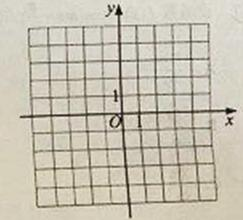
\includegraphics[width=.42\linewidth]{assets/asset-051-01.jpg}
\end{center}
\begin{solution}
\textbf{答案：}(1)图像见解析；(2)$\left(-\infty,-\frac{7}{6}\right)$

\textbf{详解：}(1)$f(x)=\begin{cases} x+3, & x\geq1\\ 5x-1, & -\frac{1}{3}<x<1\\ -x-3, & x\leq -\frac{1}{3}\end{cases}$，图像如图所示。
(2)将$f(x)$图像向左平移1个单位得$f(x+1)$图像。由图像可知，当$x$小于两图像交点横坐标时，$f(x)>f(x+1)$。解方程$-x-3=5(x+1)-1$得$x=-\frac{7}{6}$，故解集为$\left(-\infty,-\frac{7}{6}\right)$。
\end{solution}
\end{question}

\begin{question}[points=5]
\textbf{来源：}2020 年 全国I卷-文科，第 13 题\par
若 $x, y$ 满足约束条件 $\begin{cases} 2x + y - 2 \le 0, \\ x - y - 1 \ge 0, \\ y + 1 \ge 0, \end{cases}$ 则 $z = x + 7y$ 的最大值为
\fillin[{$1$}]
\begin{solution}
\textbf{答案：}$1$

\textbf{分析：}首先画出可行域，然后结合目标函数的几何意义即可求得其最大值.

\textbf{详解：}绘制不等式组表示的平面区域如图所示，目标函数 $z=x+7y$ 即 $y = -\frac{1}{7}x + \frac{1}{7}z$, 其中 $z$ 取得最大值时表示直线系在 $y$ 轴上的截距最大，据此结合目标函数的几何意义可知目标函数在点 $A$ 处取得最大值，联立直线方程 $\begin{cases} 2x+y-2=0 \\ x-y-1=0 \end{cases}$ 可得点 $A(1,0)$, 所以 $z_{\max}=1+7\times0=1$.
\end{solution}
\end{question}

\begin{question}[points=10]
\textbf{来源：}2020 年 全国I卷-文科，第 23 题\par
已知函数 $f(x) = |3x+1| - 2|x-1|$.



(1) 画出 $y = f(x)$ 的图像;



(2) 求不等式 $f(x) > f(x+1)$ 的解集.

\begin{center}
  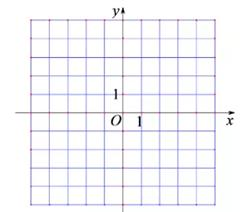
\includegraphics[width=.42\linewidth]{assets/asset-053-01.jpg}
\end{center}
\begin{solution}
\textbf{答案：}(1) 图像见解析； (2) $\left(-\infty, -\frac{7}{6}\right)$.

\textbf{分析：}(1) 根据分段讨论法，即可写出函数 $f(x)$ 的解析式，作出图象； (2) 作出函数 $f(x+1)$ 的图象，根据图象即可解出.

\textbf{详解：}(1) $f(x) = \begin{cases} x+3, & x\ge 1, \\ 5x-1, & -\frac{1}{3} < x < 1, \\ -x-3, & x\le -\frac{1}{3}. \end{cases}$ 图象如图所示.

(2) 将函数 $f(x)$ 的图象向左平移 $1$ 个单位，可得函数 $f(x+1)$ 的图象，如图所示. 由 $-x-3 = 5(x+1)-1$ 解得 $x = -\frac{7}{6}$. 所以不等式的解集为 $\left(-\infty, -\frac{7}{6}\right)$.
\end{solution}
\end{question}

\section*{2021 年}

\begin{question}[points=10]
\textbf{来源：}2021 年 全国甲卷-理科，第 23 题\par
已知函数 $f(x) = |x-2|$，$g(x) = |2x+3| - |2x-1|$．（1）画出 $y=f(x)$ 和 $y=g(x)$ 的图像；（2）若 $f(x+a) \ge g(x)$，求 $a$ 的取值范围．

\begin{center}
  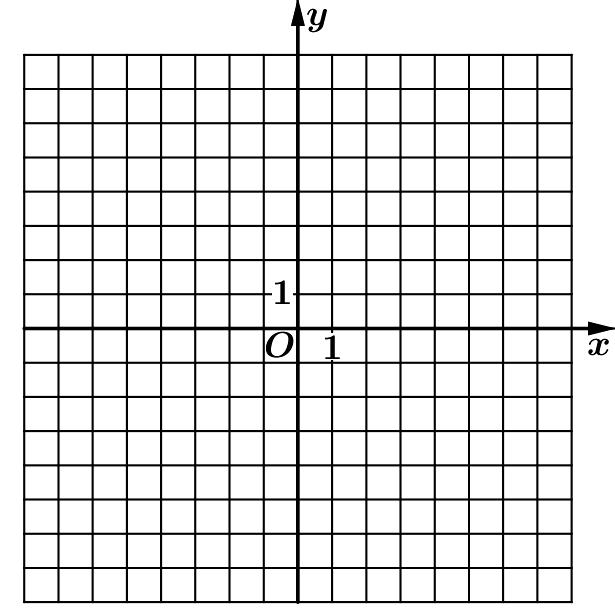
\includegraphics[width=.42\linewidth]{assets/asset-054-01.jpg}
\end{center}
\begin{solution}
\textbf{答案：}（1）图像见解析；（2）$a \ge \frac{11}{2}$

\textbf{分析：}（1）分段去绝对值即可画出图像；（2）根据函数图像数形结合可得需将 $y=f(x)$ 向左平移可满足条件，求得 $y=f(x+a)$ 过 $A(\frac{1}{2},4)$ 时 $a$ 的值可求．

\textbf{详解：}（1）$f(x)=|x-2| = \begin{cases} 2-x, & x<2 \\ x-2, & x\ge 2 \end{cases}$，$g(x)=|2x+3|-|2x-1| = \begin{cases} -4, & x<-\frac{3}{2} \\ 4x+2, & -\frac{3}{2}\le x < \frac{1}{2} \\ 4, & x\ge \frac{1}{2} \end{cases}$，图像略．（2）$f(x+a)=|x+a-2|$，由图像知需将 $f(x)$ 向左平移，即 $a>0$．当 $f(x+a)$ 过点 $A(\frac{1}{2},4)$ 时，$|\frac{1}{2}+a-2|=4$，解得 $a=\frac{11}{2}$ 或 $a=-\frac{5}{2}$（舍去），所以 $a\ge\frac{11}{2}$．
\end{solution}
\end{question}

\begin{question}[points=10]
\textbf{来源：}2021 年 全国甲卷-文科，第 23 题\par
[选修4-5：不等式选讲]



已知函数 $f(x) = |x-2|$, $g(x) = |2x+3| - |2x-1|$.



（1）画出 $y=f(x)$ 和 $y=g(x)$ 的图像；



（2）若 $f(x+a) \ge g(x)$, 求 $a$ 的取值范围．

\begin{center}
  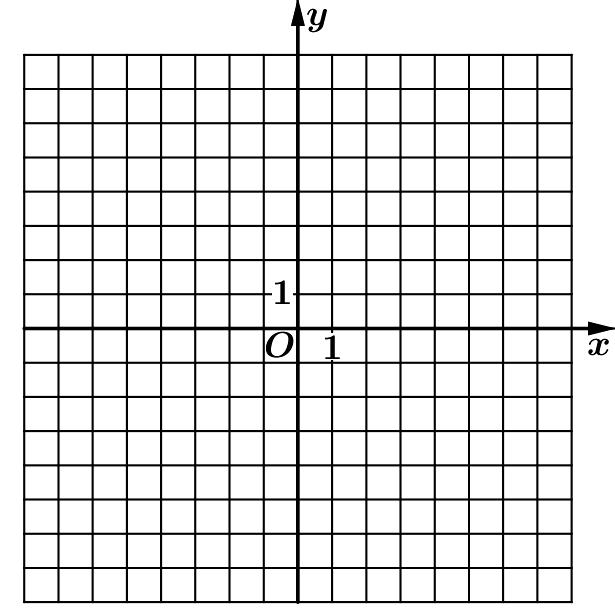
\includegraphics[width=.42\linewidth]{assets/asset-055-01.jpg}
\end{center}
\begin{solution}
\textbf{答案：}（1）图像见解析；（2）$a \ge \frac{11}{2}$.

\textbf{分析：}（1）分段去绝对值即可画出图像；（2）根据函数图像数形结合可得需将 $y=f(x)$ 向左平移可满足条件，求得 $y=f(x+a)$ 过 $A\left(\frac{1}{2},4\right)$ 时 $a$ 的值可求.

\textbf{详解：}（1）$f(x) = |x-2| = \begin{cases} 2-x, & x<2 \\ x-2, & x\ge 2 \end{cases}$, 画出图像如下：

$g(x) = |2x+3| - |2x-1| = \begin{cases} -4, & x<-\frac{3}{2} \\ 4x+2, & -\frac{3}{2} \le x < \frac{1}{2} \\ 4, & x\ge \frac{1}{2} \end{cases}$, 画出函数图像如下：

（2）$f(x+a) = |x+a-2|$, 如图，在同一个坐标系里画出 $f(x)$, $g(x)$ 图像, $y=f(x+a)$ 是 $y=f(x)$ 平移了 $a$ 个单位得到，则要使 $f(x+a) \ge g(x)$, 需将 $y=f(x)$ 向左平移，即 $a>0$. 当 $y=f(x+a)$ 过 $A\left(\frac{1}{2},4\right)$ 时, $|\frac{1}{2}+a-2| = 4$, 解得 $a = \frac{11}{2}$ 或 $a = -\frac{5}{2}$（舍去）. 则数形结合可得需至少将 $y=f(x)$ 向左平移 $\frac{11}{2}$ 个单位, 所以 $a \ge \frac{11}{2}$.
\end{solution}
\end{question}

\begin{question}[points=10]
\textbf{来源：}2021 年 全国乙卷-理科，第 23 题\par
已知函数$f(x)=|x-a|+|x+3|$。

（1）当$a=1$时，求不等式$f(x)\geq6$的解集；

（2）若$f(x)\geq -a$，求$a$的取值范围。
\begin{solution}
\textbf{答案：}（1）$(-\infty,-4]\cup[2,+\infty)$；（2）$\left(-\frac32,+\infty\right)$

\textbf{详解：}（1）当$a=1$时，$f(x)\geq6\Leftrightarrow|x-1|+|x+3|\geq6$。当$x\leq-3$时，不等式$\Leftrightarrow1-x-x-3\geq6$，解得$x\leq-4$；当$-3<x<1$时，不等式$\Leftrightarrow1-x+x+3\geq6$，解得$x\in\varnothing$；当$x\geq1$时，不等式$\Leftrightarrow x-1+x+3\geq6$，解得$x\geq2$。综上，原不等式的解集为$(-\infty,-4]\cup[2,+\infty)$。
（2）若$f(x)\geq -a$，即$f(x)_{\min}\geq -a$，因为$f(x)=|x-a|+|x+3|\geq|(x-a)-(x+3)|=|a+3|$（当且仅当$(x-a)(x+3)\leq0$时，等号成立），所以$f(x)_{\min}=|a+3|$，所以$|a+3|\geq -a$，即$a+3\leq a$或$a+3\geq -a$，解得$a\in\left(-\frac32,+\infty\right)$。
\end{solution}
\end{question}

\begin{question}[points=5]
\textbf{来源：}2021 年 全国乙卷-文科，第 5 题\par
若 $x,y$ 满足约束条件 $\begin{cases} x + y \ge 4, \\ x - y \le 2, \\ y \le 3, \end{cases}$ 则 $z = 3x + y$ 的最小值为（ ）
\begin{choices}
  \item $18$
  \item $10$
  \item $6$
  \item $4$
\end{choices}
\begin{solution}
\textbf{答案：}C

\textbf{分析：}根据约束条件可得图像如下， $z = 3x + y$ 的最小值，即 $y = -3x + z$ ， $y$ 轴截距最小值.根据图像可知 $y = -3x + z$ 过点 $B(1,3)$ 时满足题意，即 $z_{\min} = 3 + 3 = 6$ .
\end{solution}
\end{question}

\begin{question}[points=5]
\textbf{来源：}2021 年 全国乙卷-文科，第 8 题\par
下列函数中最小值为4的是（ ）
\begin{choices}
  \item $y = x^2 + 2x + 4$
  \item $y = |\sin x| + \frac{4}{|\sin x|}$
  \item $y = 2^x + 2^{2-x}$
  \item $y = \ln x + \frac{4}{\ln x}$
\end{choices}
\begin{solution}
\textbf{答案：}C

\textbf{分析：}对于 A，$y = x^2 + 2x + 4 = (x+1)^2 + 3 \ge 3$ .不符合，
对于 B，$y = |\sin x| + \frac{4}{|\sin x|}$ ，令 $t = |\sin x| \in [0,1]$ ，$y = t + \frac{4}{t}$ ，根据对勾函数 $y_{\min} = 1 + 4 = 5$ 不符合，
对于 C，$y = 2^x + 2^{2-x} = 2^x + \frac{4}{2^x}$ ，令 $t = 2^x > 0$ ，$y = t + \frac{4}{t} \ge 2\sqrt{t \cdot \frac{4}{t}} = 4$ ，当且仅当 $t=2$ 时取等，符合，
对于 D，$y = \ln x + \frac{4}{\ln x}$ ，令 $t = \ln x \in \mathbb{R}$ ，$y = t + \frac{4}{t}$ ，根据对勾函数 $y \in (-\infty, -4] \cup [4, +\infty)$ ，不符合.
\end{solution}
\end{question}

\begin{question}[points=10]
\textbf{来源：}2021 年 全国乙卷-文科，第 23 题\par
已知函数 $f(x) = |x-a| + |x+3|$ .

（1）当 $a=1$ 时，求不等式 $f(x) \ge 6$ 的解集；

（2）若 $f(x) > -a$ ，求 $a$ 的取值范围.
\begin{solution}
\textbf{答案：}见解析

\textbf{详解：}（1）当 $a=1$ 时，$f(x) \ge 6 \iff |x-1| + |x+3| \ge 6$ .
当 $x \le -3$ 时，不等式 $\iff 1-x - x - 3 \ge 6$ ，解得 $x \le -4$ ；
当 $-3 < x < 1$ 时，不等式 $\iff 1-x + x + 3 \ge 6$ ，解得 $x \in \varnothing$ ；
当 $x \ge 1$ 时，不等式 $\iff x-1 + x+3 \ge 6$ ，解得 $x \ge 2$ .
综上，原不等式的解集为 $(-\infty, -4] \cup [2, +\infty)$ .
（2）若 $f(x) > -a$ ，即 $f(x)_{\min} > -a$ ，
因为 $f(x) = |x-a| + |x+3| \ge |(x-a) - (x+3)| = |a+3|$ （当且仅当 $(x-a)(x+3) \le 0$ 时，等号成立），
所以 $f(x)_{\min} = |a+3|$ ，所以 $|a+3| > -a$ ，即 $a+3 < a$ 或 $a+3 > -a$ ，解得 $a \in \left(-\frac{3}{2}, +\infty\right)$ .
\end{solution}
\end{question}

\begin{question}[points=4]
\textbf{来源：}2021 年 上海春季卷，第 4 题\par
不等式 $\frac{2x+5}{x-2}<1$ 的解集为  .
\fillin[{$(-7,2)$}]
\begin{solution}
\textbf{答案：}$(-7,2)$

\textbf{分析：}由已知进行转化 $\frac{x+7}{x-2}<0$，进行可求．

\textbf{详解：}由 $\frac{2x+5}{x-2}<1$ 得 $\frac{2x+5}{x-2}-1<0$，即 $\frac{x+7}{x-2}<0$，解得 $-7<x<2$．故答案为 $(-7,2)$．
\end{solution}
\end{question}

\begin{question}[points=4]
\textbf{来源：}2021 年 上海春季卷，第 6 题\par
若方程组 $\begin{cases} a_1x+b_1y=c_1 \\ a_2x+b_2y=c_2 \end{cases}$ 无解，则 $\begin{vmatrix} a_1 & b_1 \\ a_2 & b_2 \end{vmatrix}=$  .
\fillin[{$0$}]
\begin{solution}
\textbf{答案：}$0$

\textbf{分析：}利用二元一次方程组的解的行列式表示进行分析即可得到答案．

\textbf{详解：}对于方程组 $\begin{cases} a_1x+b_1y=c_1 \\ a_2x+b_2y=c_2 \end{cases}$，有 $D=\begin{vmatrix} a_1 & b_1 \\ a_2 & b_2 \end{vmatrix}, D_x=\begin{vmatrix} c_1 & b_1 \\ c_2 & b_2 \end{vmatrix}, D_y=\begin{vmatrix} a_1 & c_1 \\ a_2 & c_2 \end{vmatrix}$，当 $D\neq 0$ 时，方程组的解为 $\begin{cases} x=\frac{D_x}{D} \\ y=\frac{D_y}{D} \end{cases}$，根据题意，方程组无解，所以 $D=0$，即 $\begin{vmatrix} a_1 & b_1 \\ a_2 & b_2 \end{vmatrix}=0$．
\end{solution}
\end{question}

\begin{question}[points=5]
\textbf{来源：}2021 年 上海卷，第 7 题\par
已知$\begin{cases}x\le 3\\2x-y-2\ge 0\\3x+y-8\ge 0\end{cases}$,目标函数$z=x-y$，则$z$的最大值为．
\fillin[{$4$}]
\begin{solution}
\textbf{答案：}$4$

\textbf{分析：}作出不等式表示的平面区域，根据$z$的几何意义求最值.

\textbf{详解：}如图，可行域的三个顶点为：$(3,4)$、$(2,2)$，$(3,-1)$，结合直线方程与$z$的几何意义，得$x=3$，$y=-1$，则$z_{\max}=4$；当$x=3$, $y=-1$, $z_{\max}=4$
\end{solution}
\end{question}

\begin{question}[points=5]
\textbf{来源：}2021 年 天津卷，第 13 题\par
若 $a > 0$，$b > 0$，则 $\frac{1}{a} + \frac{a}{b^2} + b$ 的最小值为.
\fillin[{$2\sqrt{2}$}]
\begin{solution}
\textbf{答案：}$2\sqrt{2}$

\textbf{分析：}两次利用基本不等式即可求出.

\textbf{详解：}$\because a>0, b>0$，$\therefore \frac{1}{a} + \frac{a}{b^2} + b \ge 2\sqrt{\frac{1}{a} \cdot \frac{a}{b^2}} + b = \frac{2}{b} + b \ge 2\sqrt{\frac{2}{b} \cdot b} = 2\sqrt{2}$，当且仅当 $\frac{1}{a} = \frac{a}{b^2}$ 且 $\frac{2}{b} = b$，即 $a=b=\sqrt{2}$ 时取等，所以最小值为 $2\sqrt{2}$.
\end{solution}
\end{question}

\begin{question}[points=4]
\textbf{来源：}2021 年 浙江卷，第 5 题\par
若实数 $x,y$ 满足约束条件 $\begin{cases} x+1 \geq 0 \\ x-y \leq 0 \\ 2x+3y-1 \leq 0 \end{cases}$, 则 $z = x - \frac{1}{2}y$ 的最小值是（   ）
\begin{choices}
  \item $-2$
  \item $-\frac{3}{2}$
  \item $-\frac{1}{2}$
  \item $\frac{1}{10}$
\end{choices}
\begin{solution}
\textbf{答案：}B

\textbf{分析：}画出可行域, 目标函数化为 $y=2x-2z$, 求过可行域点且斜率为2的直线在 y 轴上截距的最大值.

\textbf{详解：}可行域如图, 由 $\begin{cases} x=-1 \\ 2x+3y-1=0 \end{cases}$ 得 $A(-1,1)$. 当直线 $y=2x-2z$ 过 $A$ 点时, $z$ 取最小值 $z = -1 - \frac{1}{2}\times1 = -\frac{3}{2}$.
\end{solution}
\end{question}

\section*{2022 年}

\begin{question}[points=10]
\textbf{来源：}2022 年 全国甲卷-理科，第 23 题\par
已知a, b, c均为正数，且 $a^2+b^2+4c^2=3$，证明:

(1) $a+b+2c\leq 3$;

(2) 若 $b=2c$，则 $\frac{1}{a}+\frac{1}{c}\geq 3$.
\begin{solution}
\textbf{答案：}(1) 证明见解析；(2) 证明见解析

\textbf{分析：}(1) 方法一：根据 $a^2+b^2+4c^2=a^2+b^2+(2c)^2$，利用柯西不等式即可得证. (2) 由(1)结合已知可得 $0<a+4c\leq 3$，即可得到 $\frac{1}{a+4c}\geq \frac{1}{3}$，再根据权方和不等式即可得证.

\textbf{详解：}(1) 由柯西不等式有 $[a^2+b^2+(2c)^2](1^2+1^2+1^2)\geq (a+b+2c)^2$，所以 $a+b+2c\leq 3$，当且仅当 $a=b=2c=1$ 时取等号，所以 $a+b+2c\leq 3$.
(2) 因为 $b=2c$, $a>0$, $b>0$, $c>0$，由(1)得 $a+b+2c=a+4c\leq 3$，即 $0<a+4c\leq 3$，所以 $\frac{1}{a+4c}\geq \frac{1}{3}$. 由权方和不等式知 $\frac{1}{a}+\frac{1}{c}=\frac{1}{a}+\frac{2}{2c}\geq \frac{(1+\sqrt{2})^2}{a+2c}=\frac{(1+\sqrt{2})^2}{a+\frac{b}{2}}$? 注意 $b=2c$，则 $c=\frac{b}{2}$，且 $b=2c$，所以 $c=\frac{b}{2}$，而 $b$ 是变量，这里需改用另一形式：$\frac{1}{a}+\frac{1}{c}=\frac{1^2}{a}+\frac{1^2}{c}\geq \frac{(1+1)^2}{a+c}=\frac{4}{a+c}$，但 $a+c$ 与 $a+4c$ 不同，需重新推导：由 $b=2c$ 及条件 $a^2+b^2+4c^2=3$ 得 $a^2+4c^2+4c^2=3$，即 $a^2+8c^2=3$，且 $a+4c\leq 3$，但目标为 $\frac{1}{a}+\frac{1}{c}\geq 3$，可考虑用柯西不等式：$(\frac{1}{a}+\frac{1}{c})(a+4c)=(\frac{1}{a}+\frac{1}{c})(a+4c)\geq (1+2)^2=9$，所以 $\frac{1}{a}+\frac{1}{c}\geq \frac{9}{a+4c}\geq \frac{9}{3}=3$，当且仅当 $\frac{1}{a}:\frac{1}{c}=a:4c$ 即 $a=2c$ 且 $b=2c$ 时取等号，此时 $a=2c$, $a^2+8c^2=4c^2+8c^2=12c^2=3$，得 $c=\frac{1}{2}$, $a=1$，等号成立. 故 $\frac{1}{a}+\frac{1}{c}\geq 3$.
\end{solution}
\end{question}

\begin{question}[points=10]
\textbf{来源：}2022 年 全国甲卷-文科，第 23 题\par
[选修4-5：不等式选讲]

已知 $a,b,c$ 均为正数，且 $a^2+b^2+4c^2=3$，证明：

（1）$a+b+2c\le3$；

（2）若 $b=2c$，则 $\frac{1}{a}+\frac{1}{c}\ge3$．
\begin{solution}
\textbf{答案：}（1）证明见解析；（2）证明见解析
\end{solution}
\end{question}

\begin{question}[points=10]
\textbf{来源：}2022 年 全国乙卷-理科，第 23 题\par
[选修4-5：不等式选讲]

已知$a,b,c$都是正数，且$a^{\frac{3}{2}}+b^{\frac{3}{2}}+c^{\frac{3}{2}}=1$，证明：

(1)$abc\leq\frac{1}{9}$；

(2)$\frac{a}{b+c}+\frac{b}{a+c}+\frac{c}{a+b}\leq\frac{1}{2\sqrt{abc}}$．
\begin{solution}
\textbf{答案：}见解析

\textbf{分析：}(1)利用三元均值不等式即可证明；(2)利用基本不等式及不等式的性质证明即可．

\textbf{详解：}【小问1详解】证明：因为$a>0,b>0,c>0$，则$a^{\frac{3}{2}}>0,b^{\frac{3}{2}}>0,c^{\frac{3}{2}}>0$，所以$a^{\frac{3}{2}}+b^{\frac{3}{2}}+c^{\frac{3}{2}}\geq 3\sqrt[3]{a^{\frac{3}{2}}b^{\frac{3}{2}}c^{\frac{3}{2}}}$，即$(abc)^{\frac{1}{2}}\leq\frac{1}{3}$，所以$abc\leq\frac{1}{9}$，当且仅当$a^{\frac{3}{2}}=b^{\frac{3}{2}}=c^{\frac{3}{2}}$即$a=b=c=\sqrt[3]{\frac{1}{9}}$时取等号．\\【小问2详解】证明：因为$a>0,b>0,c>0$，所以$b+c\geq 2\sqrt{bc}$，$a+c\geq 2\sqrt{ac}$，$a+b\geq 2\sqrt{ab}$，所以$\frac{a}{b+c}\leq\frac{a}{2\sqrt{bc}}=\frac{a^{\frac{3}{2}}}{2\sqrt{abc}}$，$\frac{b}{a+c}\leq\frac{b}{2\sqrt{ac}}=\frac{b^{\frac{3}{2}}}{2\sqrt{abc}}$，$\frac{c}{a+b}\leq\frac{c}{2\sqrt{ab}}=\frac{c^{\frac{3}{2}}}{2\sqrt{abc}}$，\\$\frac{a}{b+c}+\frac{b}{a+c}+\frac{c}{a+b}\leq\frac{a^{\frac{3}{2}}+b^{\frac{3}{2}}+c^{\frac{3}{2}}}{2\sqrt{abc}}=\frac{1}{2\sqrt{abc}}$当且仅当$a=b=c$时取等号．
\end{solution}
\end{question}

\begin{question}[points=5]
\textbf{来源：}2022 年 全国乙卷-文科，第 5 题\par
若 $x, y$ 满足约束条件 $\begin{cases} x+y \ge 2 \\ x+2y \le 4 \\ y \ge 0 \end{cases}$, 则 $z = 2x - y$ 的最大值是
\begin{choices}
  \item $-2$
  \item 4
  \item 8
  \item 12
\end{choices}
\begin{solution}
\textbf{答案：}C

\textbf{分析：}作出可行域，数形结合即可得解.

\textbf{详解：}由题意作出可行域，如图阴影部分所示. 转化目标函数 $z=2x-y$ 为 $y=2x-z$, 上下平移直线，当直线过点 $(4,0)$ 时，截距最小，$z$ 最大，所以 $z_{\max}=2\times4-0=8$.
\end{solution}
\end{question}

\begin{question}[points=10]
\textbf{来源：}2022 年 全国乙卷-文科，第 23 题\par
[选修4-5：不等式选讲]

已知 $a,b,c$ 都是正数，且 $a^{\frac32}+b^{\frac32}+c^{\frac32}=1$, 证明：

(1) $abc \le \frac19$;

(2) $\frac{a}{b+c}+\frac{b}{a+c}+\frac{c}{a+b} \le \frac{1}{2\sqrt{abc}}$.
\begin{solution}
\textbf{答案：}证明见解析.

\textbf{分析：}(1) 利用三元均值不等式.
(2) 利用基本不等式放缩.

\textbf{详解：}(1) 由 $a^{\frac32}+b^{\frac32}+c^{\frac32} \ge 3\sqrt[3]{a^{\frac32}b^{\frac32}c^{\frac32}} = 3(abc)^{\frac12}$ 得 $1 \ge 3(abc)^{\frac12}$, 所以 $abc \le \frac19$.
(2) 由 $b+c\ge2\sqrt{bc}$ 得 $\frac{a}{b+c} \le \frac{a}{2\sqrt{bc}} = \frac{a^{\frac32}}{2\sqrt{abc}}$, 同理 $\frac{b}{a+c} \le \frac{b^{\frac32}}{2\sqrt{abc}}$, $\frac{c}{a+b} \le \frac{c^{\frac32}}{2\sqrt{abc}}$, 相加得 $\frac{a}{b+c}+\frac{b}{a+c}+\frac{c}{a+b} \le \frac{a^{\frac32}+b^{\frac32}+c^{\frac32}}{2\sqrt{abc}} = \frac{1}{2\sqrt{abc}}$.
\end{solution}
\end{question}

\begin{question}[points=5]
\textbf{来源：}2022 年 上海卷，第 2 题\par
若实数$a$、$b$满足$a>b>0$，下列不等式中恒成立的是（ ）
\begin{choices}
  \item $a+b>2\sqrt{ab}$
  \item $a+b<2\sqrt{ab}$
  \item $\frac{a}{2}+2b>2\sqrt{ab}$
  \item $\frac{a}{2}+2b<2\sqrt{ab}$
\end{choices}
\begin{solution}
\textbf{答案：}A

\textbf{分析：}利用已知条件以及基本不等式化简即可判断求解．

\textbf{详解：}解：因为$a>b>0$，所以$a+b\geq 2\sqrt{ab}$，当且仅当$a=b$时取等号，又$a>b>0$，所以$a+b>2\sqrt{ab}$，故 A 正确，B 错误；$\frac{a}{2}+2b\geq 2\sqrt{\frac{a}{2}\cdot 2b}=2\sqrt{ab}$，当且仅当$\frac{a}{2}=2b$，即$a=4b$时取等号，故 CD 错误，故选：A．
\end{solution}
\end{question}

\begin{question}[points=4]
\textbf{来源：}2022 年 上海卷，第 5 题\par
$x-y\leq 0$，$x+y-1\geq 0$，求$z=x+2y$的最小值 ．
\fillin[{$\frac{3}{2}$}]
\begin{solution}
\textbf{答案：}$\frac{3}{2}$

\textbf{分析：}根据已知条件作出可行域，再求目标函数的最小值即可．

\textbf{详解：}解：如图所示：由$x-y\leq 0$，$x+y-1\geq 0$，可知可行域为直线$x-y=0$的左上方和$x+y-1=0$的右上方的公共部分，联立$\begin{cases}x-y=0\\x+y-1=0\end{cases}$，可得$\begin{cases}x=\frac{1}{2}\\y=\frac{1}{2}\end{cases}$，即图中点$A\left(\frac{1}{2},\frac{1}{2}\right)$，当目标函数$z=x+2y$沿着与正方向向量$\vec{v}=(1,2)$的相反向量平移时，离开区间时取最小值，即目标函数$z=x+2y$过点$A\left(\frac{1}{2},\frac{1}{2}\right)$时，取最小值：$\frac{1}{2}+2\times\frac{1}{2}=\frac{3}{2}$．故答案为：$\frac{3}{2}$．
\end{solution}
\end{question}

\begin{question}[points=5]
\textbf{来源：}2022 年 新高考II卷，第 12 题\par
若$x,y$满足$x^2+y^2-xy=1$，则（ ）
\begin{choices}
  \item $x+y\leq 1$
  \item $x+y\geq -2$
  \item $x^2+y^2\leq 2$
  \item $x^2+y^2\geq 1$
\end{choices}
\begin{solution}
\textbf{答案：}BC

\textbf{分析：}根据基本不等式或者取特值即可判断各选项的真假.

\textbf{详解：}因为$ab\leq\left(\dfrac{a+b}{2}\right)^2\leq\dfrac{a^2+b^2}{2}$（$a,b\in\mathbf{R}$），由$x^2+y^2-xy=1$可变形为$(x+y)^2-1=3xy\leq 3\left(\dfrac{x+y}{2}\right)^2$，解得$-2\leq x+y\leq 2$，当且仅当$x=y=-1$时，$x+y=-2$，当且仅当$x=y=1$时，$x+y=2$，所以A错误，B正确；由$x^2+y^2-xy=1$可变形为$x^2+y^2-1=xy\leq\dfrac{x^2+y^2}{2}$，解得$x^2+y^2\leq 2$，当且仅当$x=y=\pm1$时取等号，所以C正确；因为$x^2+y^2-xy=1$变形可得$\left(x-\dfrac{y}{2}\right)^2+\dfrac{3}{4}y^2=1$，设$x-\dfrac{y}{2}=\cos\theta,\dfrac{\sqrt{3}}{2}y=\sin\theta$，所以$x=\cos\theta+\dfrac{1}{\sqrt{3}}\sin\theta,y=\dfrac{2}{\sqrt{3}}\sin\theta$，因此$x^2+y^2=\cos^2\theta+\dfrac{5}{3}\sin^2\theta+\dfrac{2}{\sqrt{3}}\sin\theta\cos\theta=1+\dfrac{1}{\sqrt{3}}\sin2\theta-\dfrac{1}{3}\cos2\theta+\dfrac{1}{3}=\dfrac{4}{3}+\dfrac{2}{3}\sin\left(2\theta-\dfrac{\pi}{6}\right)\in\left[\dfrac{2}{3},2\right]$，所以当$x=\dfrac{\sqrt{3}}{3},y=-\dfrac{\sqrt{3}}{3}$时满足等式，但是$x^2+y^2\geq 1$不成立，所以D错误．故选BC.
\end{solution}
\end{question}

\begin{question}[points=4]
\textbf{来源：}2022 年 浙江卷，第 3 题\par
若实数 $x,y$ 满足约束条件 $\begin{cases} x-2 \ge 0, \\ 2x+y-7 \le 0, \\ x-y-2 \le 0, \end{cases}$ 则 $z = 3x+4y$ 的最大值是（ ）
\begin{choices}
  \item $20$
  \item $18$
  \item $13$
  \item $6$
\end{choices}
\begin{solution}
\textbf{答案：}B

\textbf{分析：}在平面直角坐标系中画出可行域，平移动直线 $z=3x+4y$ 后可求最大值.

\textbf{详解：}不等式组对应的可行域如图所示：当动直线 $3x+4y-z=0$ 过 $A$ 时 $z$ 有最大值．由 $\begin{cases} x=2 \\ 2x+y-7=0 \end{cases}$ 得 $A(2,3)$，故 $z_{\max}=3\times2+4\times3=18$，故选B.
\end{solution}
\end{question}

\begin{question}[points=4]
\textbf{来源：}2022 年 浙江卷，第 9 题\par
已知 $a,b \in \mathbb{R}$，若对任意 $x \in \mathbb{R}, a|x-b| + |x-4| - |2x-5| \ge 0$，则（ ）
\begin{choices}
  \item $a \le 1, b \ge 3$
  \item $a \le 1, b \le 3$
  \item $a \ge 1, b \ge 3$
  \item $a \ge 1, b \le 3$
\end{choices}
\begin{solution}
\textbf{答案：}D

\textbf{分析：}将问题转换为 $a|x-b| \ge |2x-5| - |x-4|$，再结合画图求解．

\textbf{详解：}设 $f(x)=a|x-b|$，$g(x)=|2x-5|-|x-4| = \begin{cases} 1-x, & x \le \frac{5}{2} \\ 3x-9, & \frac{5}{2} < x < 4 \\ x-1, & x \ge 4 \end{cases}$，则 $f(x)$ 的图象恒在 $g(x)$ 的上方（可重合），由图可知，$a \ge 3, 1 \le b \le 3$，或 $1 \le a < 3, 1 \le b \le 4-\frac{3}{a} \le 3$，故选D.
\end{solution}
\end{question}

\section*{2023 年}

\begin{question}[points=5]
\textbf{来源：}2023 年 全国甲卷-理科，第 14 题\par
若 $x$，$y$ 满足约束条件 $\begin{cases} 3x - 2y \le 3 \\ -2x + 3y \le 3 \\ x + y \ge 1 \end{cases}$，设 $z = 3x + 2y$ 的最大值为 ．
\fillin[{$15$}]
\begin{solution}
\textbf{答案：}$15$

\textbf{分析：}由约束条件作出可行域，根据线性规划求最值即可．

\textbf{详解：}作出可行域，如图，由图可知，当目标函数 $y = -\frac{3}{2}x + \frac{z}{2}$ 过点 $A$ 时，$z$ 有最大值，由 $\begin{cases} -2x+3y=3 \\ 3x-2y=3 \end{cases}$ 可得 $\begin{cases} x=3 \\ y=3 \end{cases}$，即 $A(3,3)$，所以 $z_{\max} = 3\times3+2\times3=15$．
\end{solution}
\end{question}

\begin{question}[points=10]
\textbf{来源：}2023 年 全国甲卷-理科，第 23 题\par
设 $a>0$，函数 $f(x) = |2x-a| - a$．

（1）求不等式 $f(x) < x$ 的解集；

（2）若曲线 $y = f(x)$ 与 $x$ 轴所围成的图形的面积为 2，求 $a$．
\begin{solution}
\textbf{答案：}（1）$(\frac{a}{3}, 3a)$；（2）$a=2$

\textbf{分析：}（1）分 $x\le a$ 和 $x>a$ 讨论即可；（2）写出分段函数，画出草图，表达面积解方程即可．

\textbf{详解：}（1）若 $x\le a$，则 $f(x)=2a-2x-a = a-2x < x$，即 $3x > a$，解得 $x > \frac{a}{3}$，即 $\frac{a}{3} < x \le a$；若 $x>a$，则 $f(x)=2x-2a-a = 2x-3a < x$，解得 $x < 3a$，即 $a < x < 3a$；综上，不等式的解集为 $(\frac{a}{3}, 3a)$．
（2）$f(x) = \begin{cases} -2x + a, & x\le a \\ 2x - 3a, & x>a \end{cases}$，画出 $f(x)$ 的草图，则 $f(x)$ 与 $x$ 轴围成 $\triangle ABC$，$\triangle ABC$ 的高为 $a$，$A(\frac{a}{2},0)$，$B(\frac{3a}{2},0)$，所以 $|AB| = a$，所以 $S_{\triangle ABC} = \frac{1}{2}|AB|\cdot a = \frac{1}{2}a^2 = 2$，解得 $a=2$．
\end{solution}
\end{question}

\begin{question}[points=5]
\textbf{来源：}2023 年 全国甲卷-文科，第 15 题\par
若 $x,y$ 满足约束条件 $\begin{cases}3x-2y\le3\\-2x+3y\le3\\x+y\ge1\end{cases}$，则 $z=3x+2y$ 的最大值为．
\fillin[{$15$}]
\begin{solution}
\textbf{答案：}$15$

\textbf{分析：}由约束条件作出可行域，根据线性规划求最值即可.

\textbf{详解：}作出可行域，如图，由图可知，当目标函数 $y=-\frac{3}{2}x+\frac{z}{2}$ 过点 $A$ 时，$z$ 有最大值，由 $\begin{cases}-2x+3y=3\\3x-2y=3\end{cases}$ 可得 $\begin{cases}x=3\\y=3\end{cases}$，即 $A(3,3)$，所以 $z_{\max}=3\times3+2\times3=15$．
\end{solution}
\end{question}

\begin{question}[points=10]
\textbf{来源：}2023 年 全国甲卷-文科，第 23 题\par
[选修4-5：不等式选讲]（10分）

已知 $f(x)=2|x-a|-a, a>0$．

（1）求不等式 $f(x)<x$ 的解集；

（2）若曲线 $y=f(x)$ 与 $x$ 轴所围成的图形的面积为2，求 $a$．
\begin{solution}
\textbf{答案：}（1）$(\frac{a}{3},3a)$；（2）$\frac{2\sqrt{6}}{3}$

\textbf{分析：}（1）分 $x\le a$ 和 $x>a$ 讨论即可；（2）写出分段函数，画出草图，表达面积解方程即可.

\textbf{详解：}（1）若 $x\le a$，则 $f(x)=2a-2x-a<x$，即 $3x>a$，解得 $x>\frac{a}{3}$，即 $\frac{a}{3}<x\le a$；若 $x>a$，则 $f(x)=2x-2a-a<x$，解得 $x<3a$，即 $a<x<3a$；综上，不等式的解集为 $(\frac{a}{3},3a)$．
（2）$f(x)=\begin{cases}-2x+a, & x\le a\\ 2x-3a, & x>a\end{cases}$，画出 $f(x)$ 的草图，则 $f(x)$ 与坐标轴围成 $\triangle ADO$ 与 $\triangle ABC$，$\triangle ABC$ 的高为 $a$，$D(0,a)$，$A(\frac{a}{2},0)$，$B(\frac{3a}{2},0)$，所以 $|AB|=a$，所以 $S_{\triangle OAD}+S_{\triangle ABC}=\frac{1}{2}\cdot OA\cdot a+\frac{1}{2}\cdot AB\cdot a=\frac{3}{4}a^2=2$，解得 $a=\frac{2\sqrt{6}}{3}$．
\end{solution}
\end{question}

\begin{question}[points=5]
\textbf{来源：}2023 年 全国乙卷-理科，第 14 题\par
若 $x$，$y$ 满足约束条件 $\begin{cases} x-3y\le -1 \\ x+2y\le 9 \\ 3x+y\ge 7 \end{cases}$，则 $z=2x-y$ 的最大值为.
\fillin[{$8$}]
\begin{solution}
\textbf{答案：}$8$

\textbf{分析：}作出可行域，转化为截距最值讨论即可.

\textbf{详解：}作出可行域如图所示：$z=2x-y$，移项得 $y=2x-z$，联立 $\begin{cases} x-3y=-1 \\ x+2y=9 \end{cases}$，解得 $\begin{cases} x=5 \\ y=2 \end{cases}$，设 $A(5,2)$，显然平移直线 $y=2x$ 使其经过点 $A$，此时截距 $-z$ 最小，则 $z$ 最大，代入得 $z=8$.
\end{solution}
\end{question}

\begin{question}[points=10]
\textbf{来源：}2023 年 全国乙卷-理科，第 23 题\par
【选修4-5】已知 $f(x)=2|x|+|x-2|$.



(1) 求不等式 $f(x)\le 6-x$ 的解集；



(2) 在直角坐标系 $xOy$ 中，求不等式组 $\begin{cases} f(x)\le y \\ x+y-6\le0 \end{cases}$ 所确定的平面区域的面积.
\begin{solution}

\textbf{详解：}(1) 依题意，$f(x)=\begin{cases} 3x-2, & x>2 \\ x+2, & 0\le x\le2 \\ -3x+2, & x<0 \end{cases}$，不等式 $f(x)\le6-x$ 化为：$\begin{cases} x>2 \\ 3x-2\le6-x \end{cases}$ 或 $\begin{cases} 0\le x\le2 \\ x+2\le6-x \end{cases}$ 或 $\begin{cases} x<0 \\ -3x+2\le6-x \end{cases}$，解得 $0\le x\le2$ 或 $-2\le x<0$，因此 $-2\le x\le2$，所以原不等式的解集为 $[-2,2]$.

(2) 作出不等式组 $\begin{cases} f(x)\le y \\ x+y-6\le0 \end{cases}$ 表示的平面区域，如图中阴影 $\triangle ABC$，由 $\begin{cases} y=-3x+2 \\ x+y=6 \end{cases}$，解得 $A(-2,8)$，由 $\begin{cases} y=x+2 \\ x+y=6 \end{cases}$，解得 $C(2,4)$，又 $B(0,2)$，$D(0,6)$，所以 $\triangle ABC$ 的面积 $S_{\triangle ABC}=\frac{1}{2}|BD|\times|x_C-x_A|=\frac{1}{2}\times|6-2|\times|2-(-2)|=8$.
\end{solution}
\end{question}

\begin{question}[points=5]
\textbf{来源：}2023 年 全国乙卷-文科，第 15 题\par
若$x,y$满足约束条件$\begin{cases}x-3y\le-1\\x+2y\le9\\3x+y\ge7\end{cases}$，则$z=2x-y$的最大值为.
\fillin[{$8$}]
\begin{solution}
\textbf{答案：}$8$

\textbf{分析：}作出可行域，转化为截距最值讨论即可.

\textbf{详解：}作出可行域如下图所示：$z=2x-y$，移项得$y=2x-z$，联立$\begin{cases}x-3y=-1\\x+2y=9\end{cases}$，解得$\begin{cases}x=5\\y=2\end{cases}$，设$A(5,2)$，显然平移直线$y=2x$使其经过点$A$，此时截距$-z$最小，则$z$最大，代入得$z=8$. 故答案为8.
\end{solution}
\end{question}

\begin{question}[points=10]
\textbf{来源：}2023 年 全国乙卷-文科，第 23 题\par
[选修4-5]（10分）

已知$f(x)=|2x|+|x-2|$.

（1）求不等式$f(x)\le6-x$的解集；

（2）在直角坐标系$xOy$中，求不等式组$\begin{cases}f(x)\le y\\x+y-6\le0\end{cases}$所确定的平面区域的面积．
\begin{solution}

\textbf{分析：}（1）分段去绝对值符号求解不等式作答.
（2）作出不等式组表示的平面区域，再求出面积作答.

\textbf{详解：}（1）依题意，$f(x)=\begin{cases}3x-2, & x>2\\x+2, & 0\le x\le2\\-3x+2, & x<0\end{cases}$，不等式$f(x)\le6-x$化为：$\begin{cases}x>2\\3x-2\le6-x\end{cases}$或$\begin{cases}0\le x\le2\\x+2\le6-x\end{cases}$或$\begin{cases}x<0\\-3x+2\le6-x\end{cases}$，解$\begin{cases}x>2\\3x-2\le6-x\end{cases}$得无解；解$\begin{cases}0\le x\le2\\x+2\le6-x\end{cases}$得$0\le x\le2$；解$\begin{cases}x<0\\-3x+2\le6-x\end{cases}$得$-2\le x<0$，因此$-2\le x\le2$，所以原不等式的解集为$[-2,2]$.
（2）作出不等式组$\begin{cases}f(x)\le y\\x+y-6\le0\end{cases}$表示的平面区域，如图中阴影$\triangle ABC$，由$\begin{cases}y=-3x+2\\x+y=6\end{cases}$，解得$A(-2,8)$，由$\begin{cases}y=x+2\\x+y=6\end{cases}$，解得$C(2,4)$，又$B(0,2), D(0,6)$，所以$\triangle ABC$的面积$S_{\triangle ABC}=\frac{1}{2}|BD|\times|x_C-x_A|=\frac{1}{2}\times|6-2|\times|2-(-2)|=8$.
\end{solution}
\end{question}

\begin{question}[points=4]
\textbf{来源：}2023 年 上海卷，第 1 题\par
不等式 $|x-2|<1$ 的解集为
\fillin[{$(1,3)$}]
\begin{solution}
\textbf{答案：}$(1,3)$
\end{solution}
\end{question}

\begin{question}[points=4]
\textbf{来源：}2023 年 上海卷，第 6 题\par
已知当 $x>0$ 时，$x+\frac{1}{x} \ge 2$，则 $\frac{1}{x}+x$ 的最小值为
\fillin[{$2$}]
\begin{solution}
\textbf{答案：}$2$
\end{solution}
\end{question}

\begin{question}[points=4]
\textbf{来源：}2023 年 上海卷，第 13 题\par
已知 $a,b\in \mathbb{R}$，若 $a+b=1$ 且 $ab=0$，则 $a^2+b^2=$
\begin{choices}
  \item $1$
  \item $2$
  \item $0$
  \item $-1$
\end{choices}
\begin{solution}
\textbf{答案：}A
\end{solution}
\end{question}

\begin{question}[points=5]
\textbf{来源：}2023 年 上海卷，第 15 题\par
设 $a\in \mathbb{R}$，函数 $f(x)=x^2-2ax+a$ 在区间 $[0,1]$ 上的最小值为 $m$，在 $[1,2]$ 上的最小值为 $n$，当 $a$ 变化时，以下不可能的情形是().

\begin{center}
  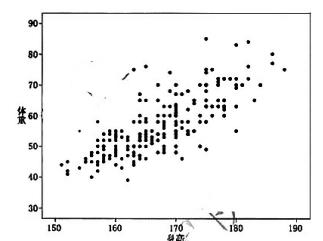
\includegraphics[width=.42\linewidth]{assets/asset-086-01.jpg}
\end{center}
\begin{choices}
  \item $m>0$ 且 $n>0$
  \item $m<0$ 且 $n<0$
  \item $m>0$ 且 $n<0$
  \item $m<0$ 且 $n>0$
\end{choices}
\begin{solution}
\textbf{答案：}D
\end{solution}
\end{question}

\section*{2024 年}

\begin{question}[points=5]
\textbf{来源：}2024 年 全国甲卷-理科，第 3 题\par
若实数 $x,y$ 满足约束条件 $\begin{cases} 4x-3y-3\ge0 \\ x-2y-2\le0 \\ 2x+6y-9\le0 \end{cases}$，则 $z=x-5y$ 的最小值为（   ）

\begin{center}
  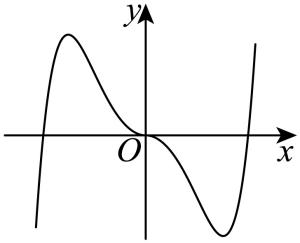
\includegraphics[width=.42\linewidth]{assets/asset-087-01.jpg}
\end{center}
\begin{choices}
  \item $5$
  \item $\dfrac{1}{2}$
  \item $-2$
  \item $-\dfrac{7}{2}$
\end{choices}
\begin{solution}
\textbf{答案：}D

\textbf{分析：}画出可行域后，利用 $z$ 的几何意义计算即可得。

\textbf{详解：}作出可行域如图，由 $z=x-5y$ 可得 $y=\frac{1}{5}x-\frac{z}{5}$，则 $z$ 的几何意义为直线 $y=\frac{1}{5}x-\frac{z}{5}$ 的截距的 $-\frac{1}{5}$，则该直线截距取最大值时，$z$ 有最小值，此时直线过点 $A$，联立 $\begin{cases}4x-3y-3=0\\2x+6y-9=0\end{cases}$，解得 $A\left(\frac{3}{2},1\right)$，则 $z_{\min}=\frac{3}{2}-5\times1=-\frac{7}{2}$。
\end{solution}
\end{question}

\begin{question}[points=10]
\textbf{来源：}2024 年 全国甲卷-理科，第 23 题\par
[选修4-5：不等式选讲]

实数 $a,b$ 满足 $a+b\ge3$。

（1）证明：$2a^2+2b^2>a+b$；

（2）证明：$|a-2b^2|+|b-2a^2|\ge6$。
\begin{solution}
\textbf{答案：}（1）证明见解析；（2）证明见解析

\textbf{分析：}（1）直接利用 $2a^2+2b^2\ge(a+b)^2$ 即可证明；（2）根据绝对值不等式并结合（1）中结论即可证明。

\textbf{详解：}（1）因为 $2a^2+2b^2-(a+b)=a^2-2ab+b^2=(a-b)^2\ge0$，当 $a=b$ 时等号成立，则 $2a^2+2b^2\ge(a+b)^2$，因为 $a+b\ge3$，所以 $2a^2+2b^2\ge(a+b)^2>a+b$。
（2）$|a-2b^2|+|b-2a^2|\ge|(a-2b^2)+(b-2a^2)|=|2a^2+2b^2-(a+b)|=2a^2+2b^2-(a+b)\ge(a+b)^2-(a+b)=(a+b)(a+b-1)\ge3\times2=6$。
\end{solution}
\end{question}

\begin{question}[points=5]
\textbf{来源：}2024 年 全国甲卷-文科，第 3 题\par
若实数 $x, y$ 满足约束条件 $\begin{cases} 4x - 3y - 3 \ge 0 \\ x - 2y - 2 \le 0 \\ 2x + 6y - 9 \le 0 \end{cases}$，则 $z = x - 5y$ 的最小值为（ ）
\begin{choices}
  \item $5$
  \item $\frac{1}{2}$
  \item $-2$
  \item $-\frac{7}{2}$
\end{choices}
\begin{solution}
\textbf{答案：}D

\textbf{分析：}画出可行域后，利用 $z$ 的几何意义计算即可得.

\textbf{详解：}实数 $x, y$ 满足约束条件，作出可行域如图（略）．由 $z = x - 5y$ 可得 $y = \frac{1}{5}x - \frac{1}{5}z$，即 $z$ 的几何意义为 $y = \frac{1}{5}x - \frac{1}{5}z$ 的截距的 $-5$，则该直线截距取最大值时，$z$ 有最小值，此时直线 $y = \frac{1}{5}x - \frac{1}{5}z$ 过点 $A$．联立 $\begin{cases} 4x - 3y - 3 = 0 \\ 2x + 6y - 9 = 0 \end{cases}$，解得 $x = \frac{3}{2}, y = 1$，即 $A(\frac{3}{2}, 1)$，则 $z_{\min} = \frac{3}{2} - 5 \times 1 = -\frac{7}{2}$.
\end{solution}
\end{question}

\begin{question}[points=10]
\textbf{来源：}2024 年 全国甲卷-文科，第 20 题\par
实数 $a, b$ 满足 $a + b \ge 3$．

（1）证明：$2a^2 + 2b^2 > a + b$；

（2）证明：$|a - 2b^2| + |b - 2a^2| \ge 6$．
\begin{solution}
\textbf{答案：}（1）见解析；（2）见解析

\textbf{分析：}（1）直接利用 $2a^2 + 2b^2 \ge (a+b)^2$ 即可证明．（2）根据绝对值不等式并结合（1）中结论即可证明.

\textbf{详解：}（1）因为 $2a^2 + 2b^2 - (a+b)^2 = a^2 - 2ab + b^2 = (a-b)^2 \ge 0$，当 $a=b$ 时等号成立，则 $2a^2 + 2b^2 \ge (a+b)^2$，因为 $a+b \ge 3$，所以 $2a^2 + 2b^2 \ge (a+b)^2 > a+b$．
（2）$|a - 2b^2| + |b - 2a^2| \ge |a - 2b^2 + b - 2a^2| = |2a^2 + 2b^2 - (a+b)| = 2a^2 + 2b^2 - (a+b) \ge (a+b)^2 - (a+b) = (a+b)(a+b-1) \ge 3 \times 2 = 6$，故原不等式成立.
\end{solution}
\end{question}

\begin{question}[points=4]
\textbf{来源：}2024 年 上海卷，第 3 题\par
已知$x\in\mathbb{R}$，则不等式$x^2-2x-3<0$的解集为.
\fillin[{$\{x\mid -1<x<3\}$}]
\begin{solution}
\textbf{答案：}$\{x\mid -1<x<3\}$

\textbf{分析：}求出方程$x^2-2x-3=0$的解后可求不等式的解集.

\textbf{详解：}方程$x^2-2x-3=0$的解为$x=-1$或$x=3$，故不等式$x^2-2x-3<0$的解集为$\{x\mid -1<x<3\}$，故答案为：$\{x\mid -1<x<3\}$.
\end{solution}
\end{question}

\section*{2025 年}

\begin{question}[points=5]
\textbf{来源：}2025 年 全国II卷，第 4 题\par
不等式 $\frac{x-4}{x-1}\ge 2$ 的解集是（ ）
\begin{choices}
  \item $\{x\mid -2\le x\le 1\}$
  \item $\{x\mid x\le -2\}$
  \item $\{x\mid -2\le x<1\}$
  \item $\{x\mid x>1\}$
\end{choices}
\begin{solution}
\textbf{答案：}$C$

\textbf{分析：}移项后转化为求一元二次不等式的解即可.

\textbf{详解：}$\frac{x-4}{x-1}\ge 2$ 即为 $\frac{x+2}{x-1}\le 0$，即 $\begin{cases}(x+2)(x-1)\le 0\\x-1\neq 0\end{cases}$，故 $-2\le x<1$，解集为 $[-2,1)$.
\end{solution}
\end{question}

\begin{question}[points=4]
\textbf{来源：}2025 年 上海卷，第 2 题\par
不等式 $\frac{x-1}{x-3} < 0$ 的解集为．
\fillin[{$(1,3)$}]
\begin{solution}
\textbf{答案：}$(1,3)$

\textbf{分析：}转化为一元二次不等式 $(x-1)(x-3) < 0$ ，解出即可.

\textbf{详解：}原不等式转化为 $(x-1)(x-3) < 0$ ，解得 $1 < x < 3$ ，则其解集为 $(1,3)$ .
\end{solution}
\end{question}

\begin{question}[points=5]
\textbf{来源：}2025 年 上海卷，第 8 题\par
设 $a, b > 0, a + \frac{1}{b} = 1$，则 $b + \frac{1}{a}$ 的最小值为．
\fillin[{$4$}]
\begin{solution}
\textbf{答案：}$4$

\textbf{分析：}灵活利用“1”将 $b + \frac{1}{a} = \left(b + \frac{1}{a}\right)\left(a + \frac{1}{b}\right)$ 展开利用基本不等式计算即可.

\textbf{详解：}易知 $b + \frac{1}{a} = \left(b + \frac{1}{a}\right)\left(a + \frac{1}{b}\right) = ab + \frac{1}{ab} + 2 \geq 2\sqrt{ab \cdot \frac{1}{ab}} + 2 = 4$，当且仅当 $ab = 1$，即 $a = \frac{1}{2}, b = 2$ 时取得最小值.
\end{solution}
\end{question}

\begin{question}[points=5]
\textbf{来源：}2025 年 天津卷，第 15 题\par
若$a, b \in \mathbb{R}$, 对$\forall x \in [-2, 2]$, 均有$(2a+b)x^2 + bx - a - 1 \le 0$恒成立, 则$2a+b$的最小值为.
\fillin[{$-4$}]
\begin{solution}
\textbf{答案：}$-4$

\textbf{分析：}先设$t = 2a + b$, 根据不等式的形式, 为了消$a$可以取$x = -\dfrac{1}{2}$, 得到$t \ge -4$, 验证$t = -4$时, $a, b$是否可以取到, 进而判断该最小值是否可取即可得到答案.

\textbf{详解：}设$t = 2a + b$, 原题转化为求$t$的最小值. 原不等式可化为对任意的$-2 \le x \le 2$, $tx^2 + (t - 2a)x - a - 1 \le 0$. 不妨代入$x = -\dfrac{1}{2}$, 得$\dfrac{1}{4}t - \dfrac{1}{2}(t - 2a) - a - 1 \le 0$, 得$t \ge -4$. 当$t = -4$时, 原不等式可化为$-4x^2 + (-4 - 2a)x - a - 1 \le 0$, 即$-\left[2x + \left(\dfrac{1}{2}a + 1\right)\right]^2 + \dfrac{1}{4}a^2 \le 0$. 观察可知, 当$a = 0$时, $-(2x+1)^2 \le 0$对$-2 \le x \le 2$一定成立, 当且仅当$x = -\dfrac{1}{2}$取等号. 此时, $a=0$, $b=-4$, 说明$t=-4$时, $a,b$均可取到, 满足题意. 故$t = 2a + b$的最小值为$-4$. 故答案为$-4$.
\end{solution}
\end{question}

